
\part*{Supplementary Information} 

\begin{figure}[hbt!]
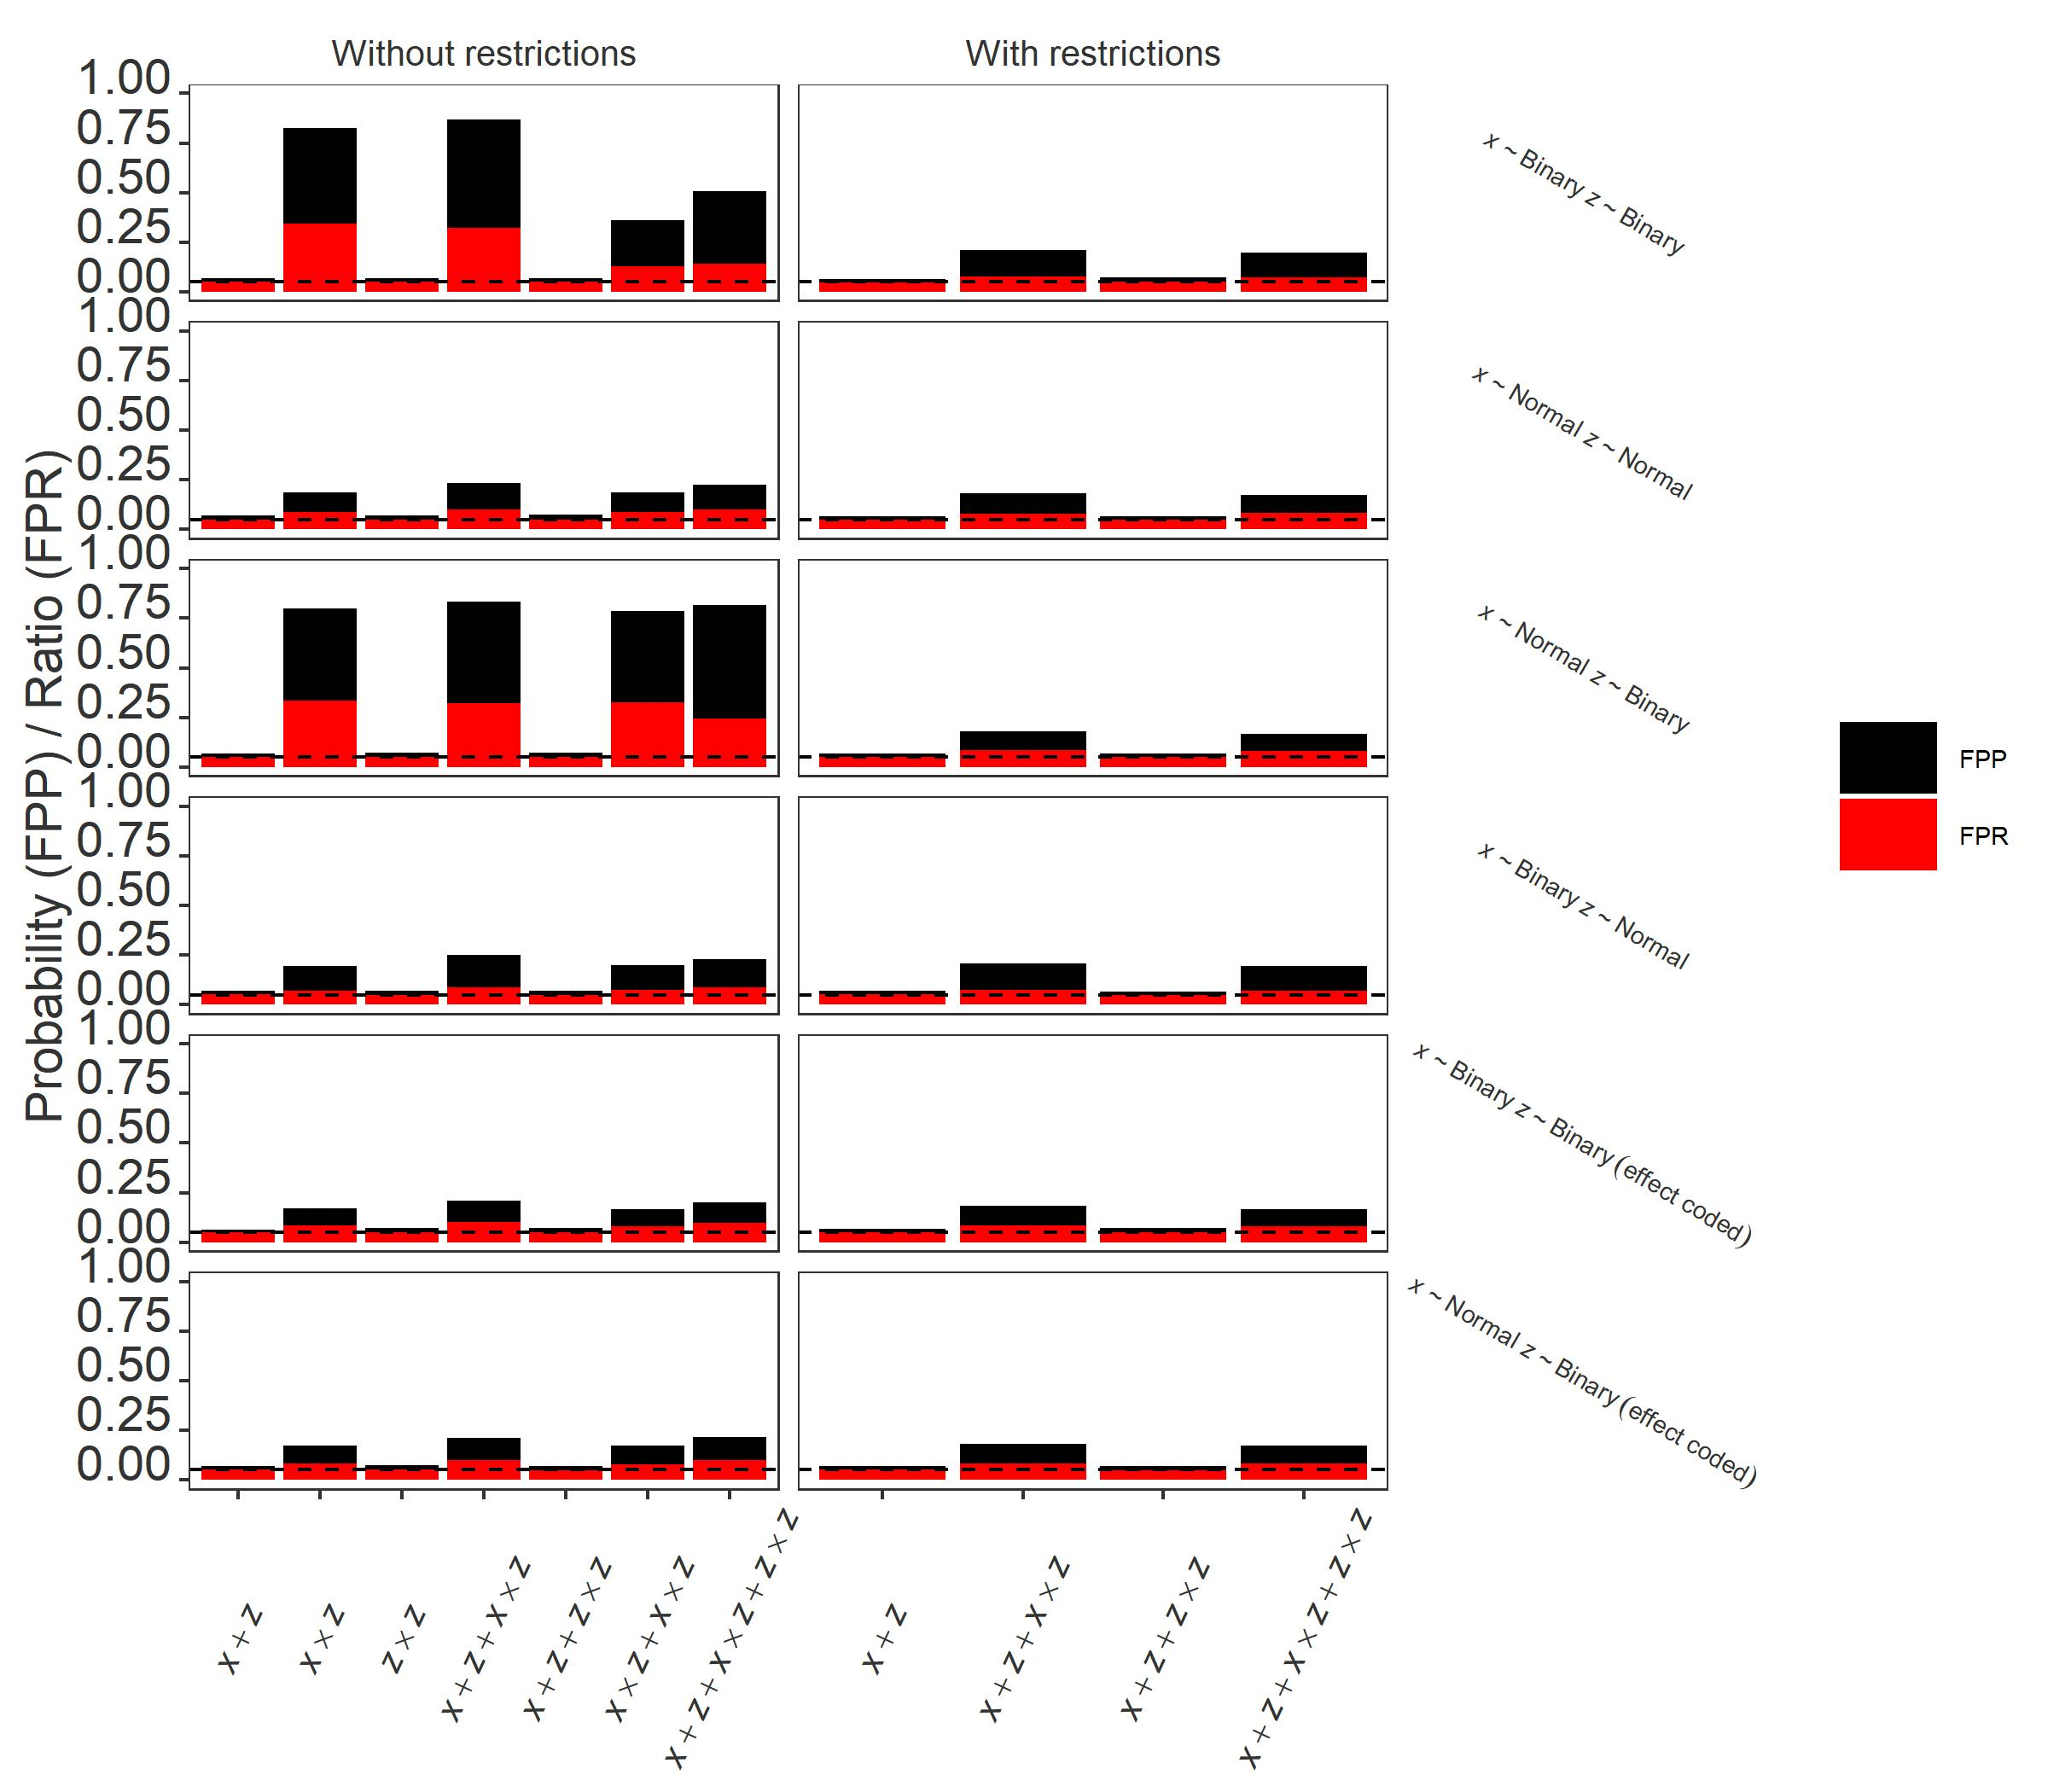
\includegraphics[scale=0.95]{R/Analysis/Result/Figures/Figure1ASI.jpeg}
\centering
\caption{The false positive probability and false positive ratio given different model sets, the presence of main effects when having interactions (i.e., With restrictions or No restrictions) and different distributions of the variable of interest and covariates. Sample size is set to 200, a correlation between the dependent variable and covariates is $\textit{r}=0.2$ and using two covariates. The false positive probability is shown in black and the false positive ratio in red. Dashed blacked line indicates 0.05. This figure adds the two other cases not shown in Figure \ref{fig:mainfigure1}}
\label{fig:appfigure1}
\end{figure}

\begin{landscape}
\begin{figure}[hbt!]
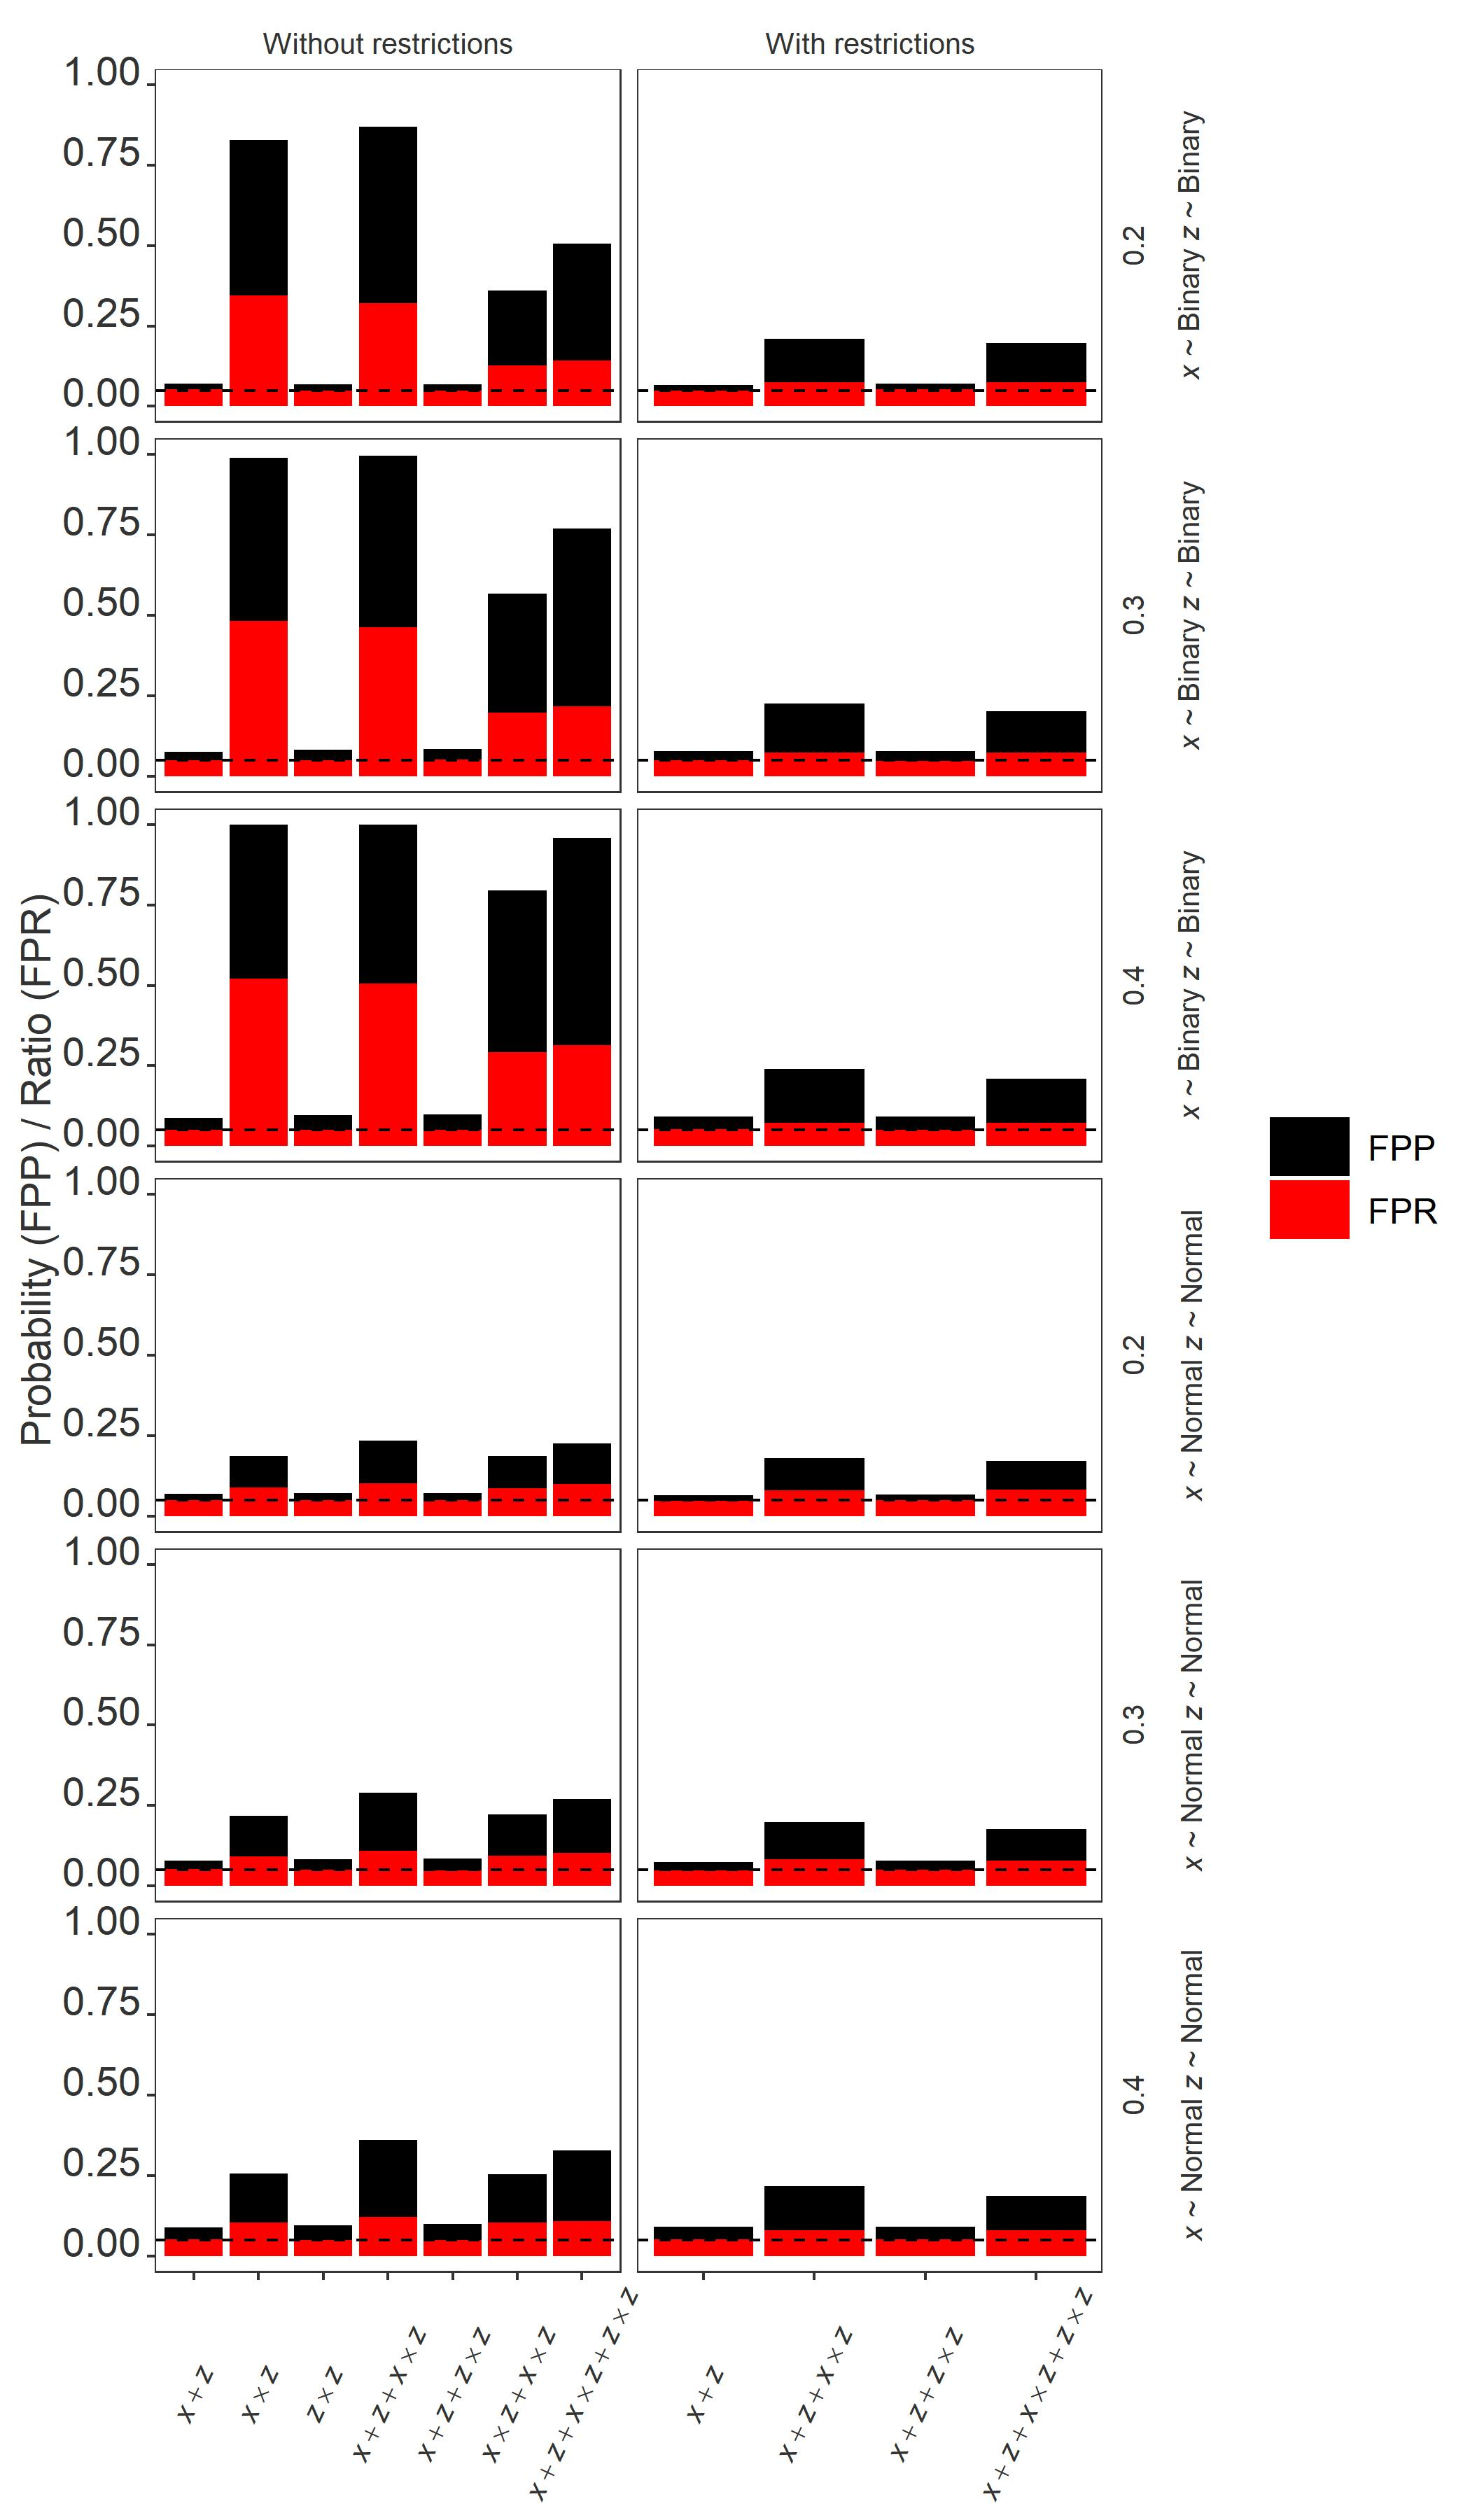
\includegraphics[scale=0.7]{R/Analysis/Result/Figures/Figure2SI.jpeg}
\centering
\caption{False positive probability and false positive for different levels of correlation between the dependent variable and the covariates ranging from  $\textit{r}=0.2$ to  $\textit{r}=0.4$. Black denotes the false positive probability and red denotes the false positive ratio. Dashed blacked line indicates 0.05. The description of the figure is otherwise the same as for Figure \ref{fig:appfigure1}.}
\label{fig:appfigure2}
\end{figure}
\end{landscape}


\begin{figure}[hbt!]
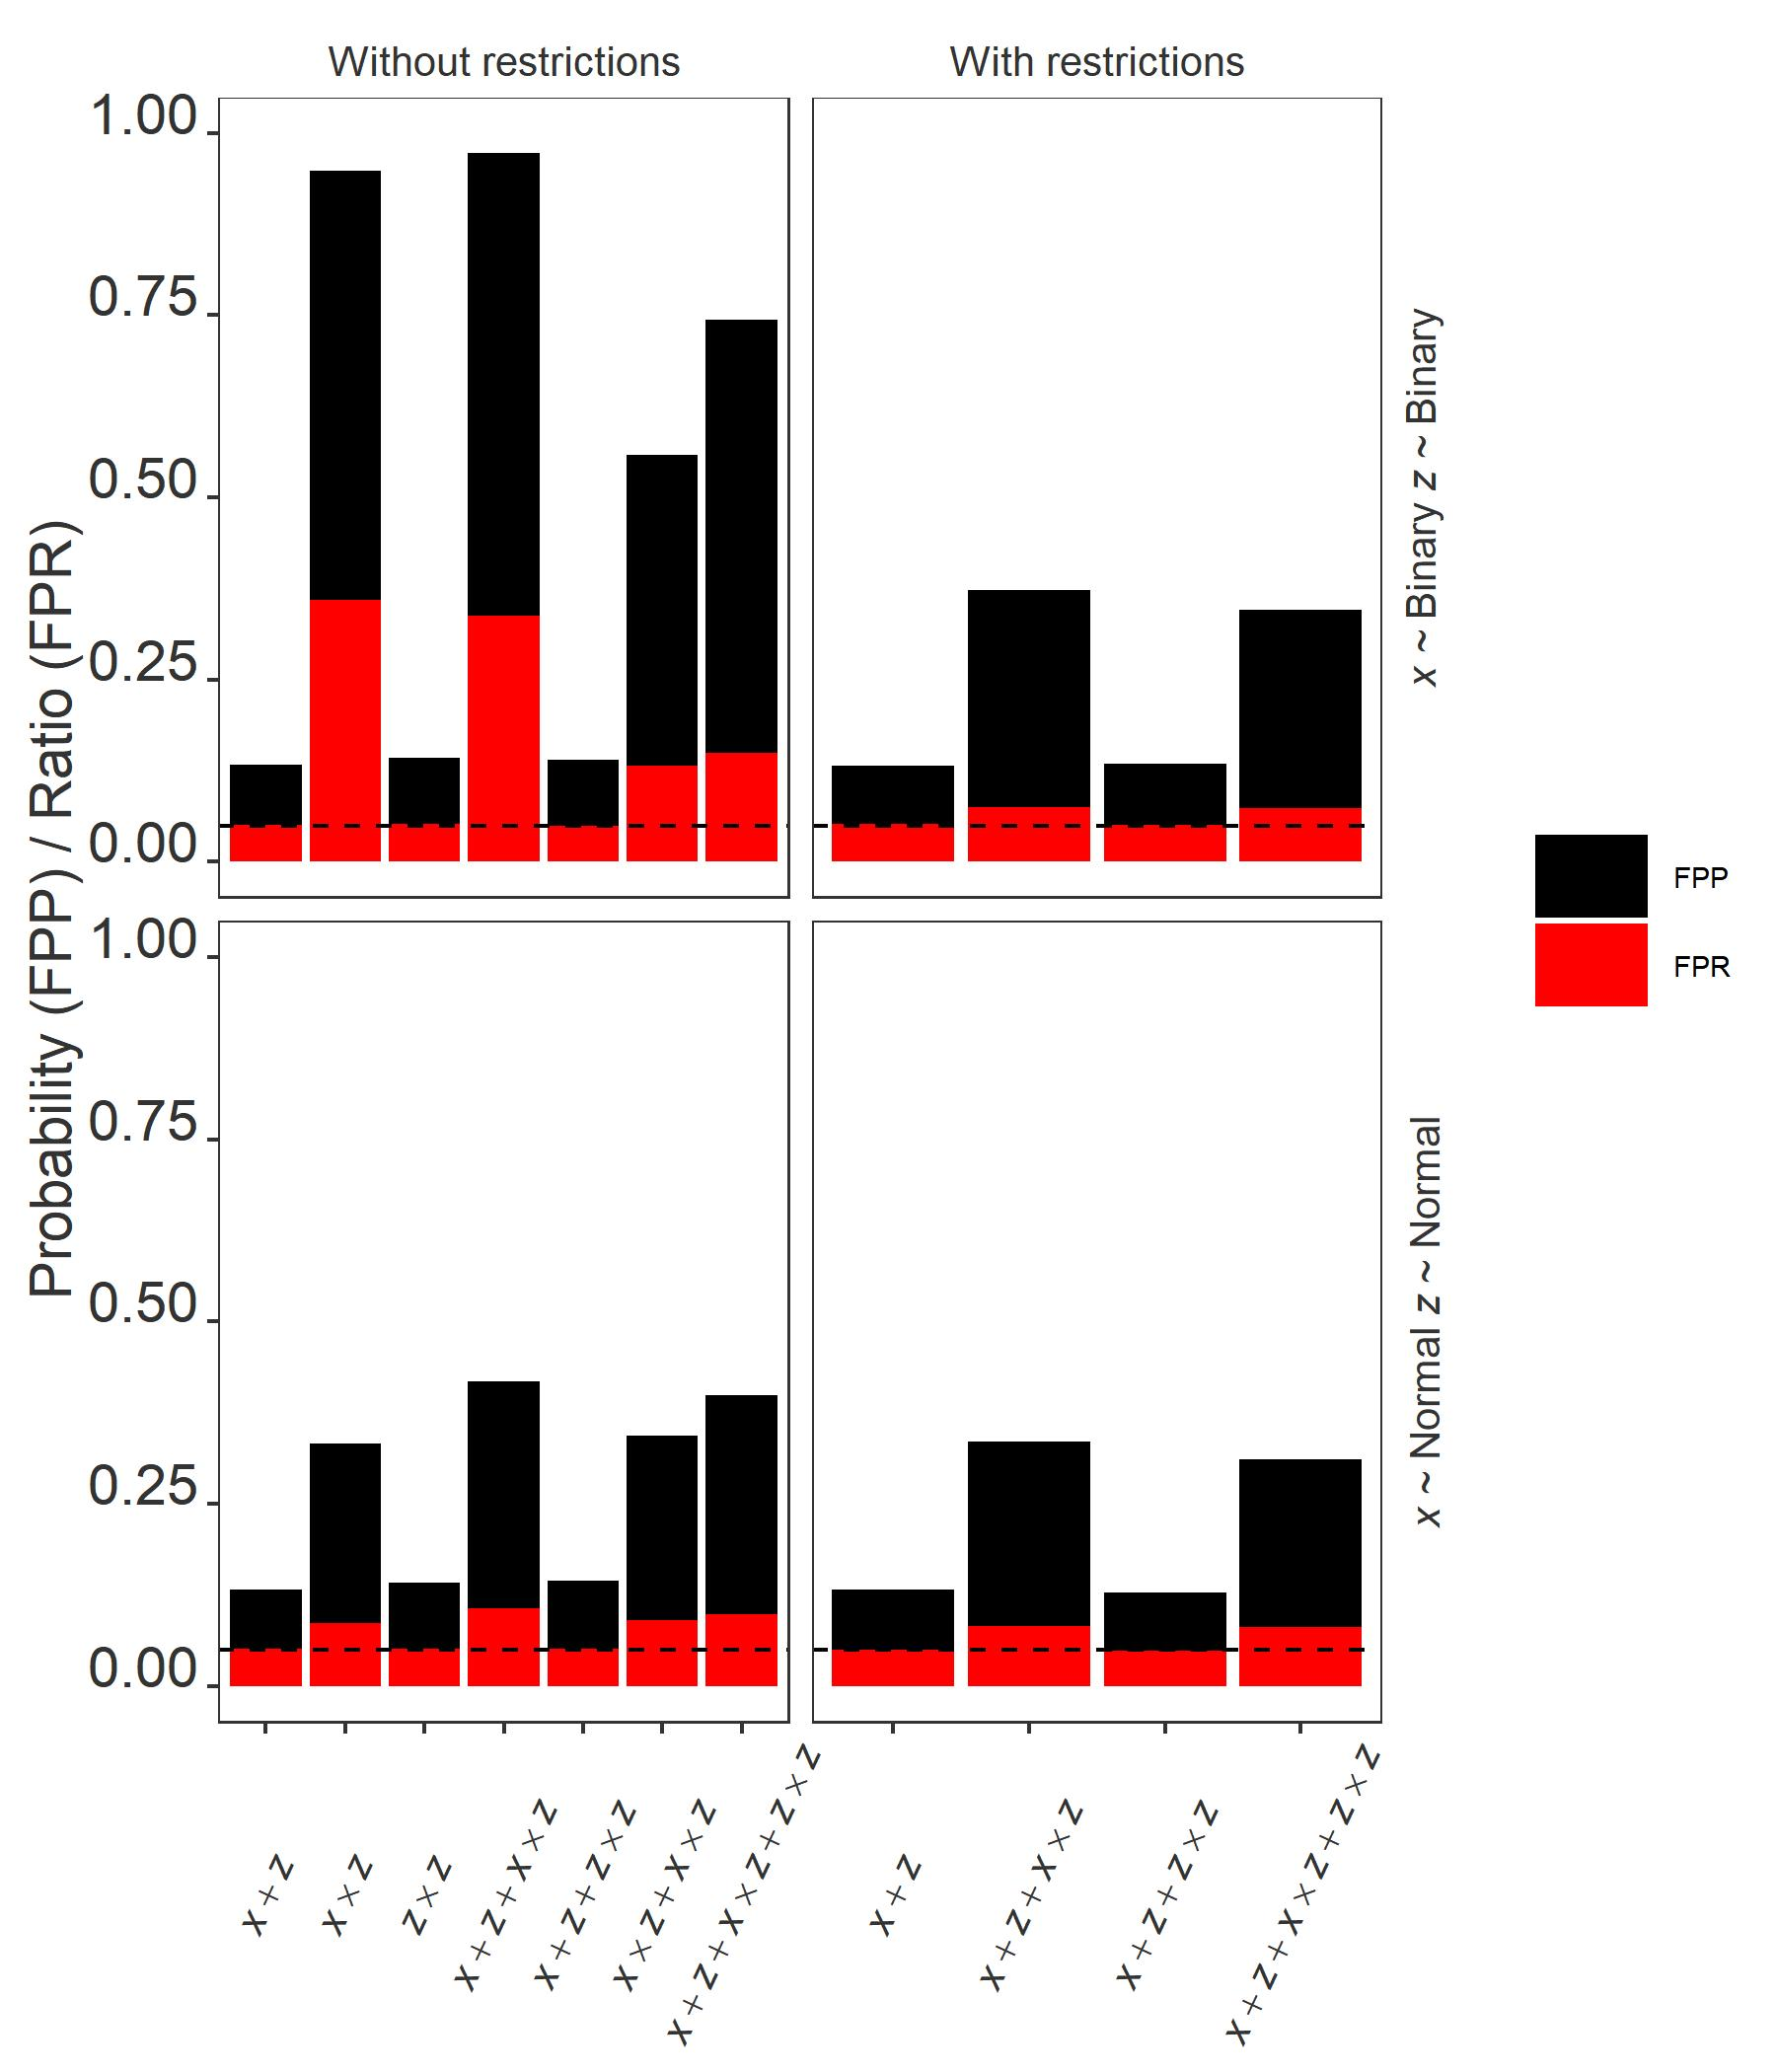
\includegraphics{R/Analysis/Result/Figures/Figure3SI.jpeg}
\centering
\caption{False positive probability and false positive ratio when using two dependent variables and the average of the two (meaning three dependent variables in total). The correlation between the dependent variables is set to  $\textit{r}=0.5$ with the correlation between the dependent variables and covariates still at  $\textit{r}=0.2$. Black denotes the the false positive probability and red denotes the false positive ratio. Dashed blacked line indicates 0.05. The description of the figure is otherwise the same as for Figure \ref{fig:appfigure1}.}
\label{fig:appfigure3}
\end{figure}


\begin{figure}[hbt!]
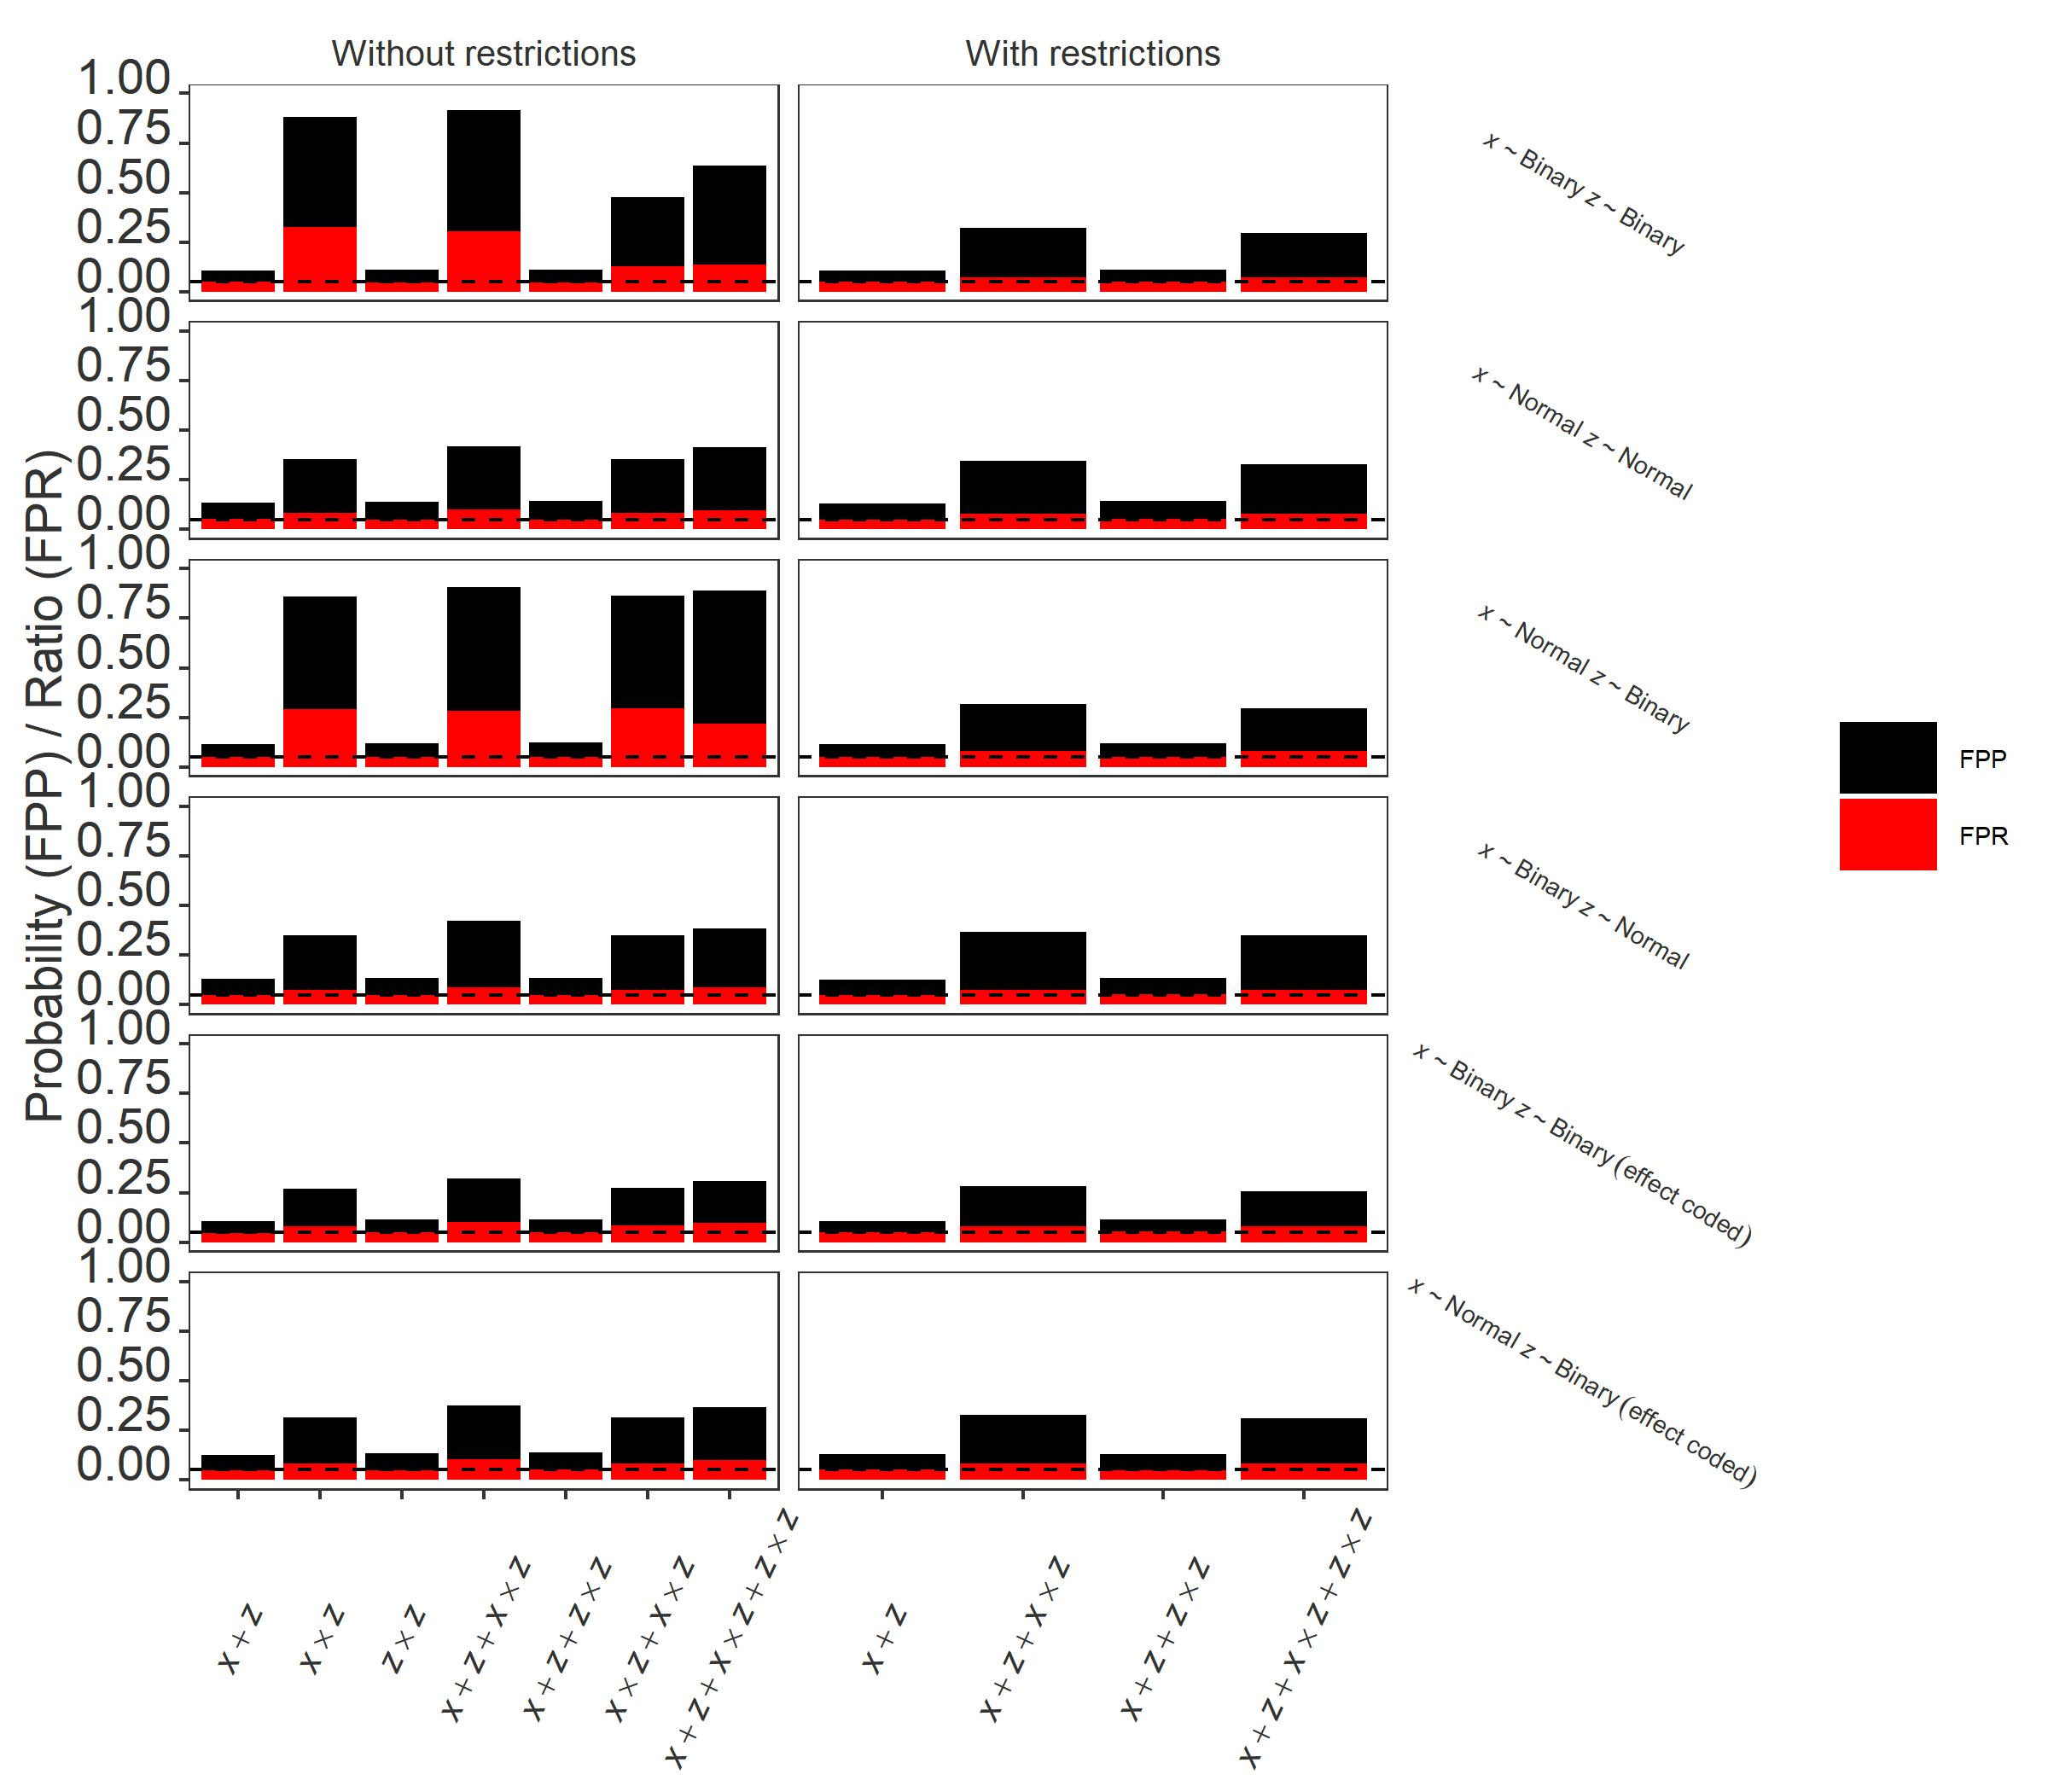
\includegraphics[scale=0.95]{R/Analysis/Result/Figures/Figure1BSI.jpeg}
\centering
\caption{False positive probability and false positive ratio when using multiple outlier criteria. Black denotes the the false positive probability and red denotes the false positive ratio. Dashed blacked line indicates 0.05. The description of the figure is otherwise the same as for Figure \ref{fig:appfigure1}. This figure adds the two other cases not shown in Figure \ref{fig:mainfigure3}.
}
\label{fig:appfigure4}
\end{figure}

\begin{figure}[hbt!]
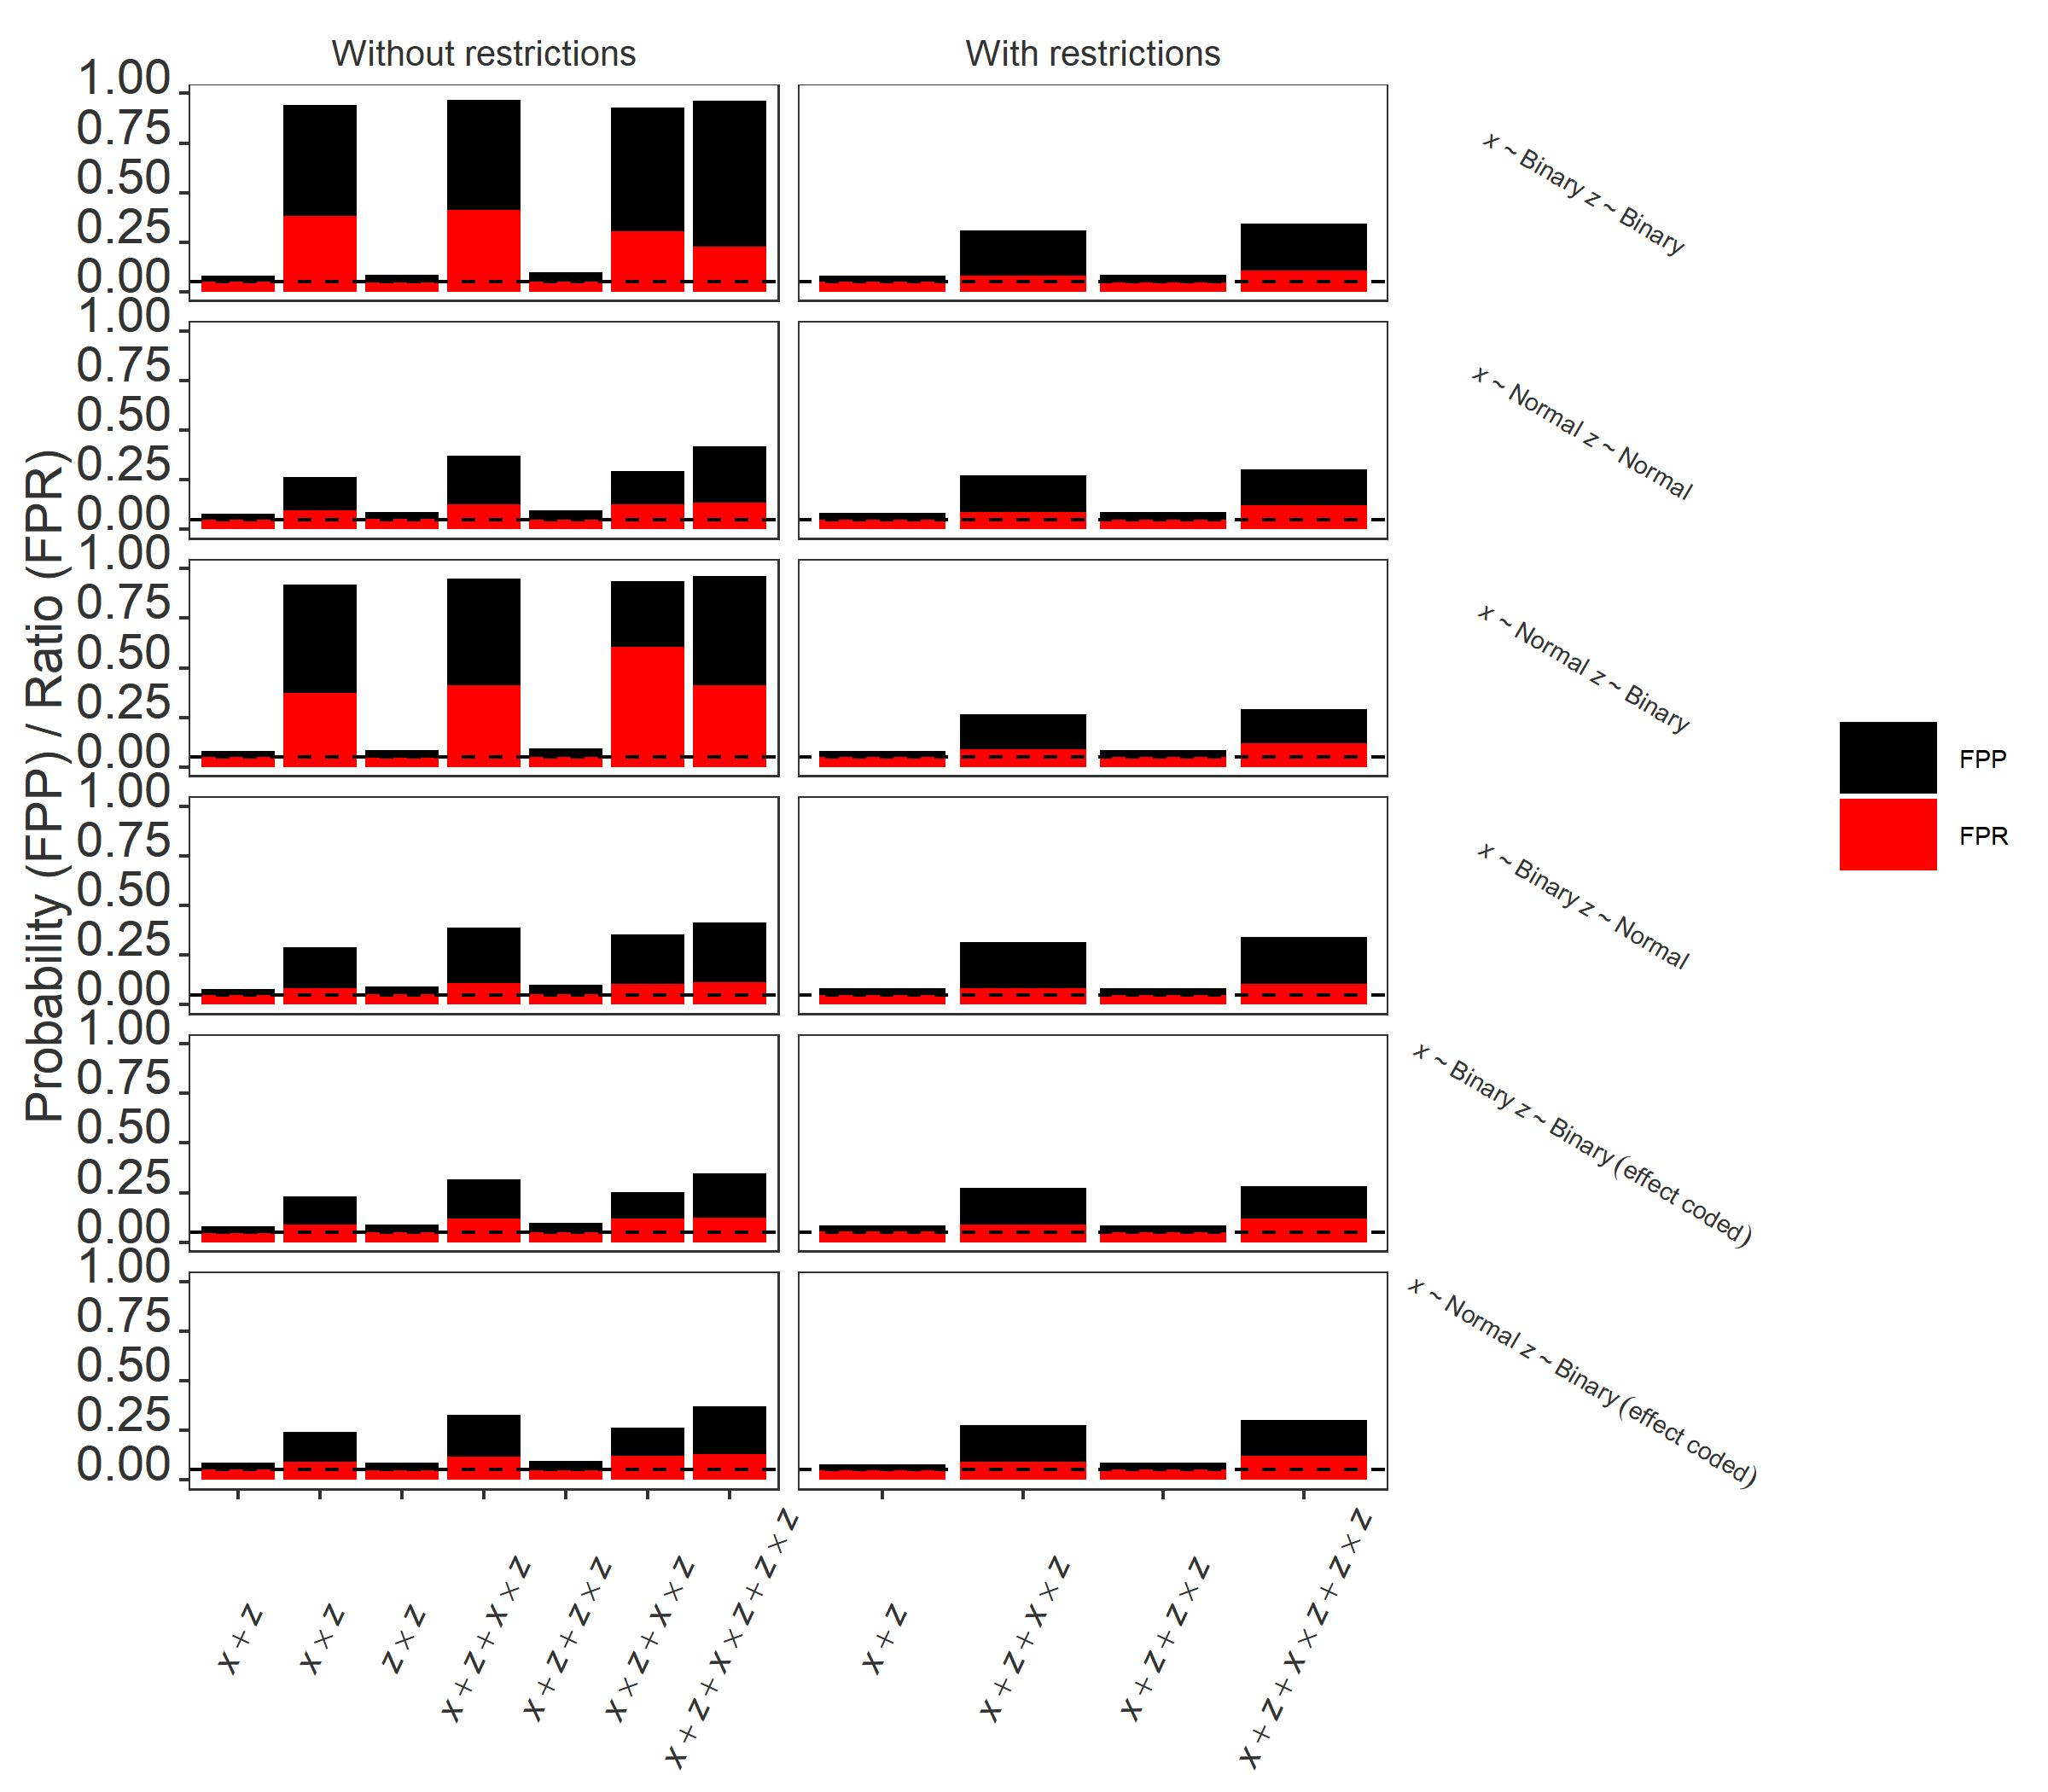
\includegraphics[scale=0.95]{R/Analysis/Result/Figures/Figure1CSI.jpeg}
\centering
\caption{False positive probability and false positive ratio when using three covariates instead of two as in the base line model. Black denotes the the false positive probability and red denotes the false positive ratio. Dashed blacked line indicates 0.05. The description of the figure is otherwise the same as for Figure \ref{fig:appfigure1}. This figure adds the two other cases not shown in Figure \ref{fig:mainfigure2}.
}
\label{fig:appfigure5}
\end{figure}

\begin{landscape}
\begin{figure}[hbt!]
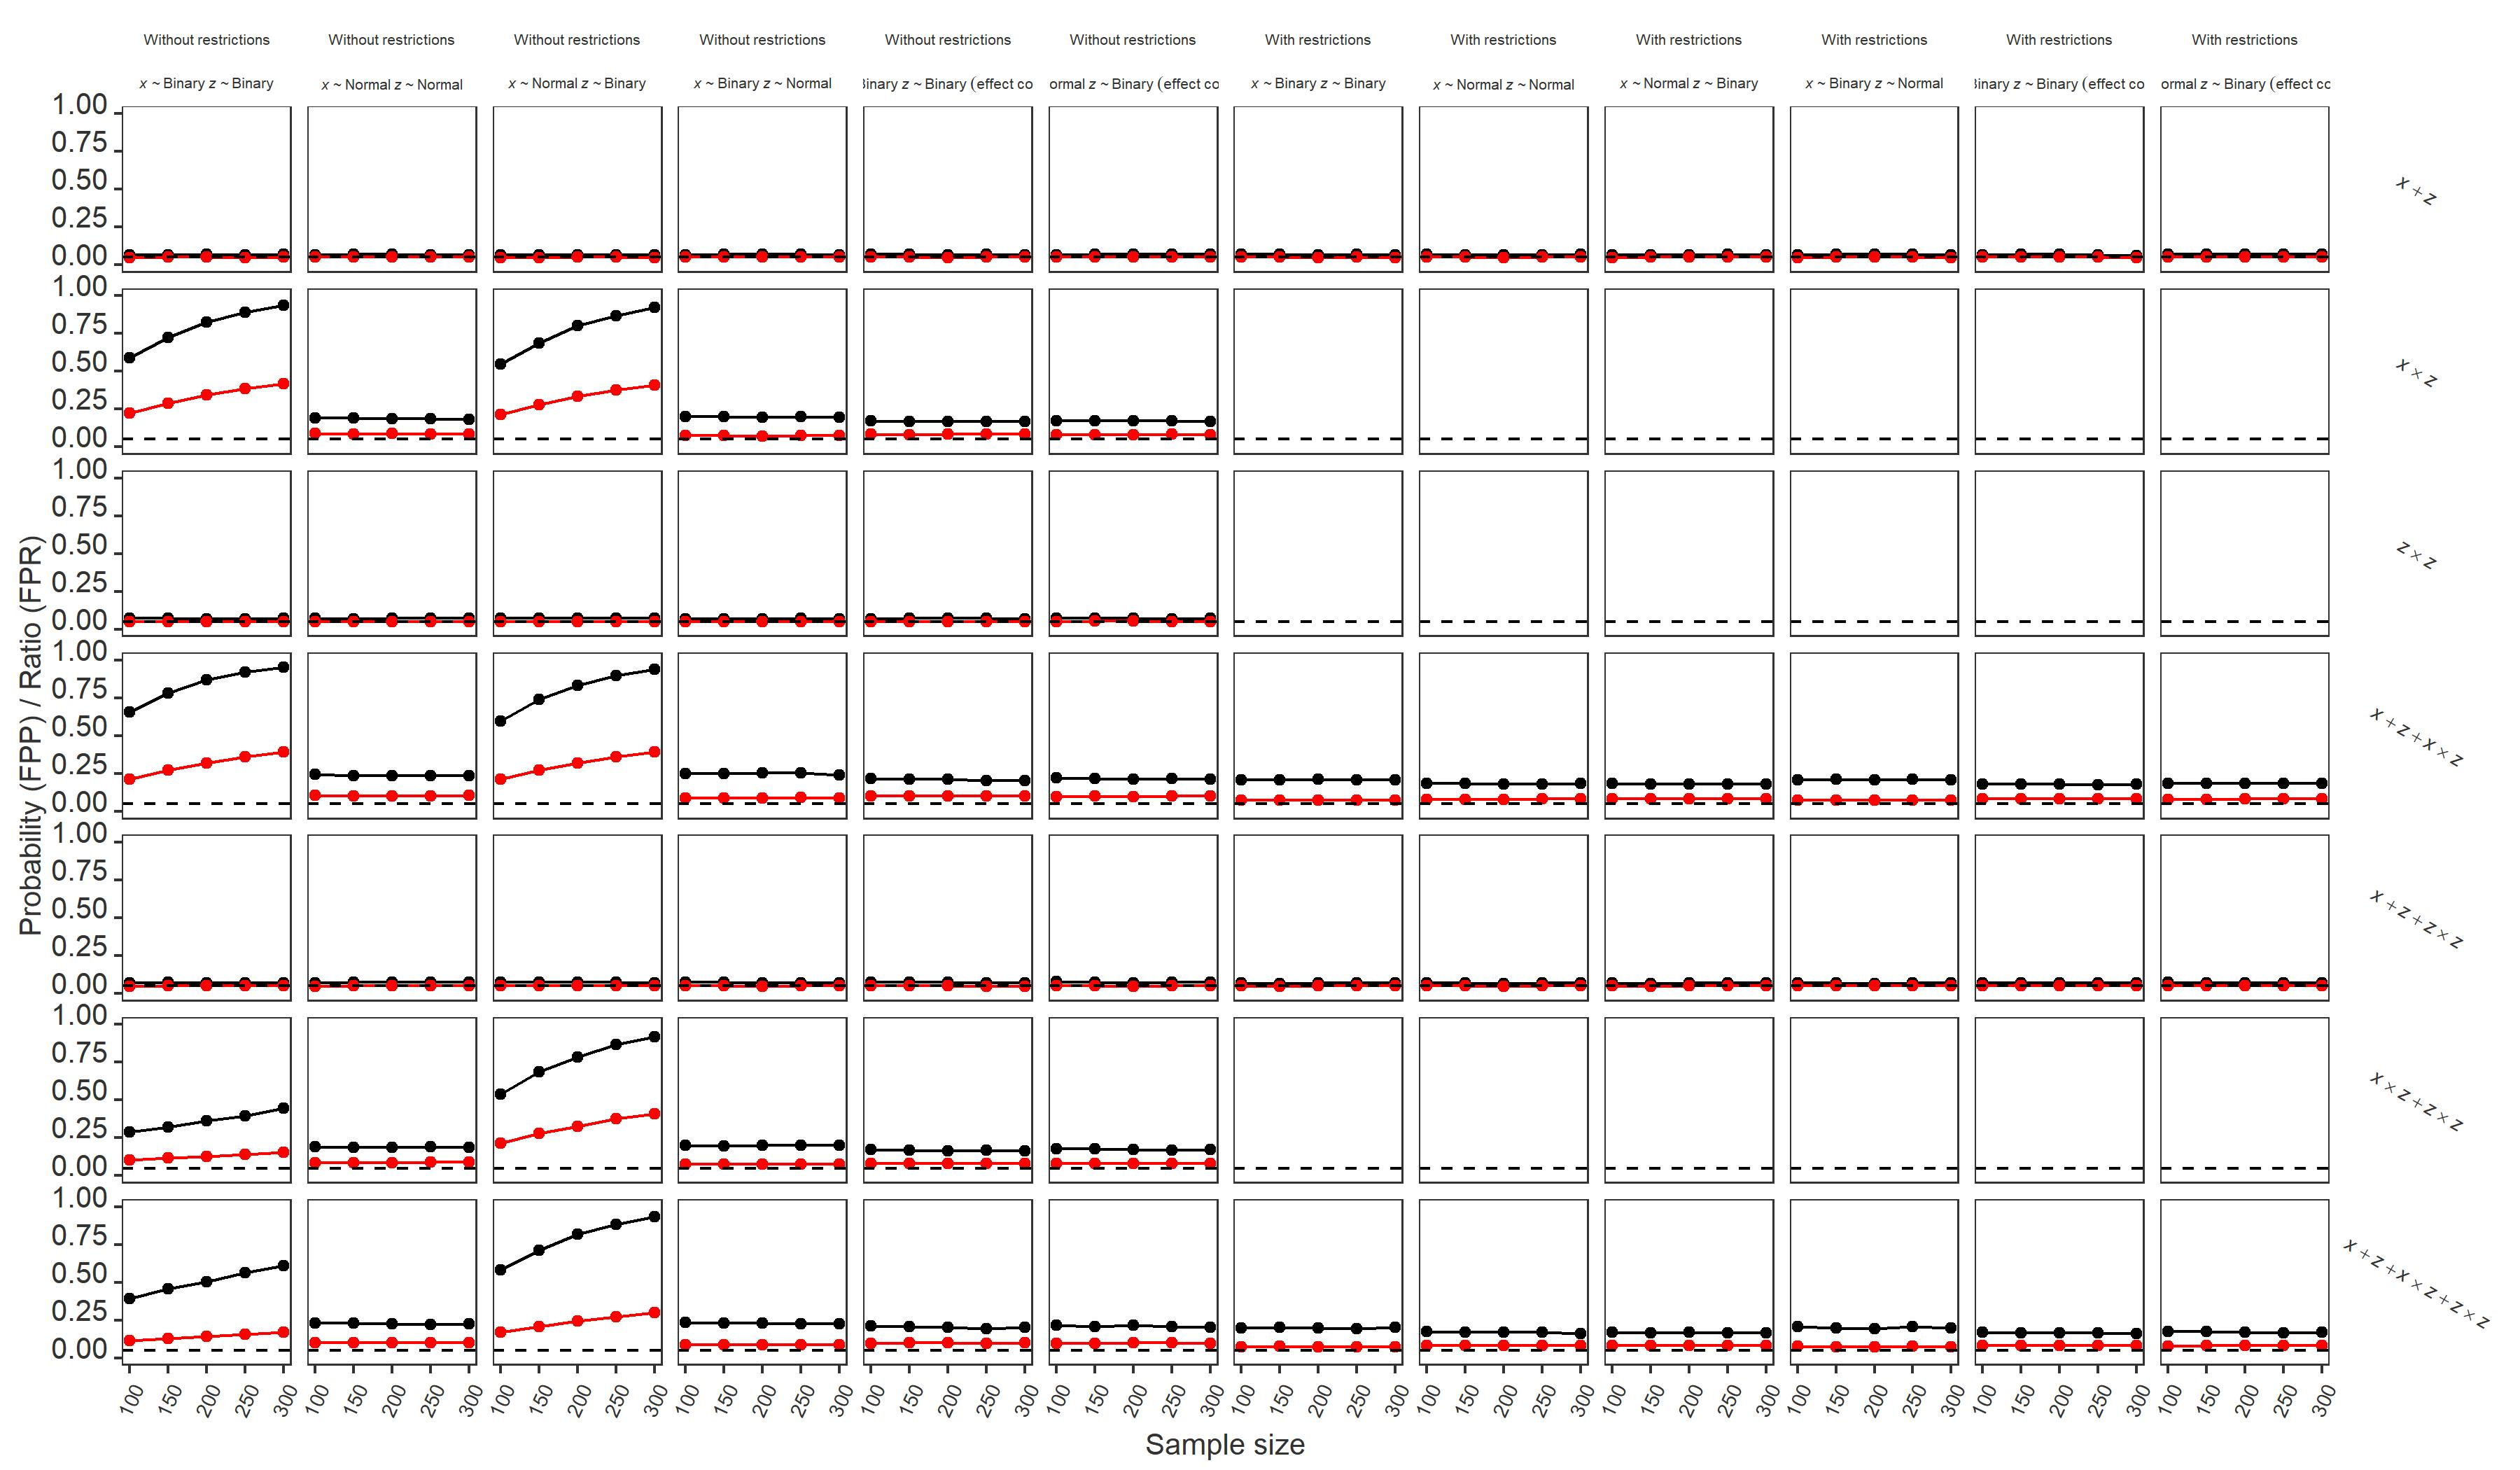
\includegraphics[scale=0.75]{R/Analysis/Result/Figures/Figure1DSI.jpeg}
\centering
\caption{Effect of increasing sample size for each model set and all combinations of data distributions (i.e., binary and normal). Black denotes the false positive probability and red denotes the false positive ratio. Dashed blacked line indicates 0.05. The description of the figure is otherwise the same as for Figure \ref{fig:appfigure1}. This figure adds the two other cases not shown in Figure \ref{fig:mainfigure4}}
\label{fig:appfigure6}
\end{figure}
\end{landscape}

\clearpage
\subsection{Results when using Bonferroni correction}

In this section, we present the same analyses but with Bonferroni correction applied. This means that the critical value ($\alpha$) now has a correction such that $\alpha = 0.05 / #Number~of~test~in~each~set$. So the critical value will only be 0.05 in the case where there is no interactions between the variable of interest and the covariates. The critical value is corrected for each test such that it can differ within each model set depending on how many interactions there are per model. 

Table \ref{tab:resultFullBC} shows the FPP and FPR for the full model sets under different conditions when there is used Bonferroni correction. Here there is no split between each model set.This lowers the FPR to the expected 5\% but there is still an issue when not including main effects and having binomial variables. 

% latex table generated in R 4.0.0 by xtable 1.8-4 package
% Wed Feb 03 15:03:29 2021
\begin{longtable}{llrr}
\caption{False positive probability (FPP) and false positive ratio (FPR) when looking at all the models possible when the sample size is 200, no outlier criteria is being used and having two covariates. When restrictions on interactions are on main effects should always be present when there is interactions, this is not the case when restrictions on interactions is off.} \\ 
  \hline
Restrictions on interactions & Type & FPP & FPR \\ 
  \hline
Without & Normal & 0.25 & 0.10 \\ 
  Without & Binomial & 0.87 & 0.23 \\ 
  With & Normal & 0.19 & 0.08 \\ 
  With & Binomial & 0.21 & 0.08 \\ 
   \hline
\hline
\end{longtable}


\begin{figure}[hbt!]
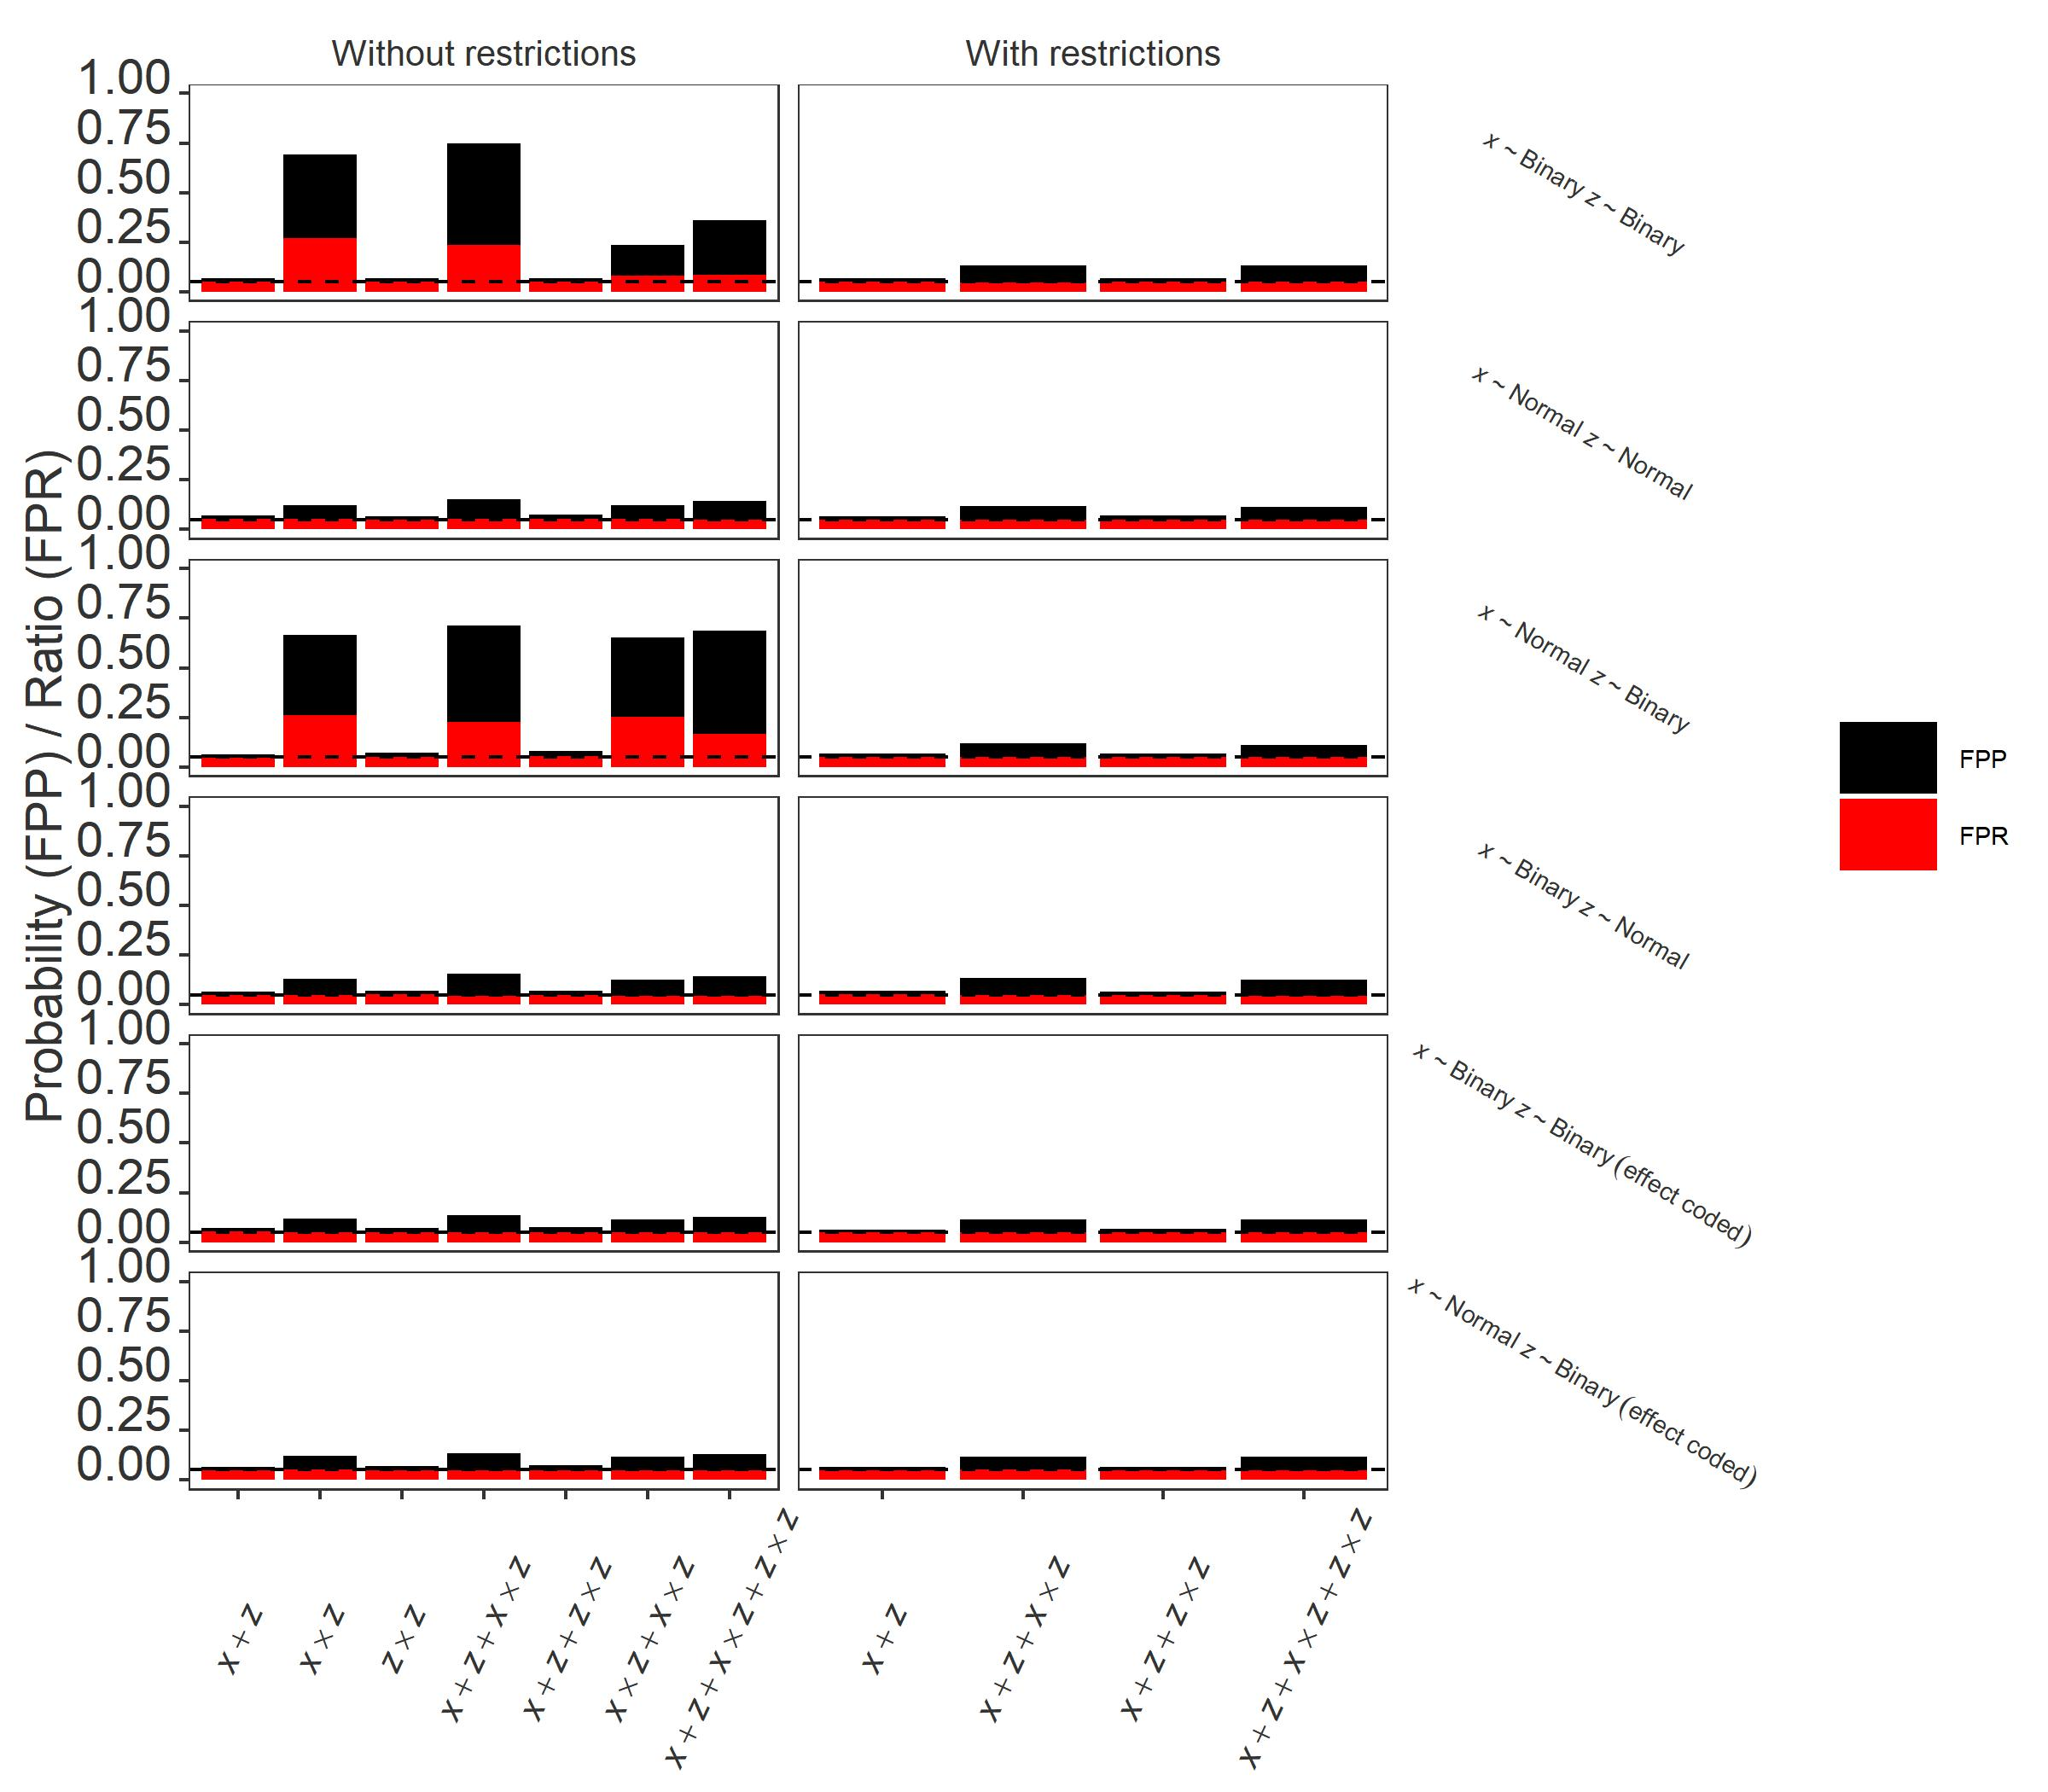
\includegraphics[scale=0.95]{R/Analysis/Result/Figures/Figure1ASIBon.jpeg}
\centering
\caption{The description of this figure is the same as for Figure \ref{fig:appfigure1} with the only difference being that we applied Bonferroni correction. This figure therefore shows the probability of the false positive probability and false positive ratio given different model sets, the presence of main effects when having interactions (i.e., With restrictions for interactions or No restrictions for interactions) and different distributions of the variable of interest and covariates. Sample size was set to 200, a correlation between the dependent variable and covariates was $\textit{r}=0.2$ and we used two covariates. The false positive probability is shown in black and the false positive ratio in red. Dashed blacked line indicates 0.05. }
\label{fig:appfigure7}
\end{figure}

\begin{landscape}
\begin{figure}[hbt!]
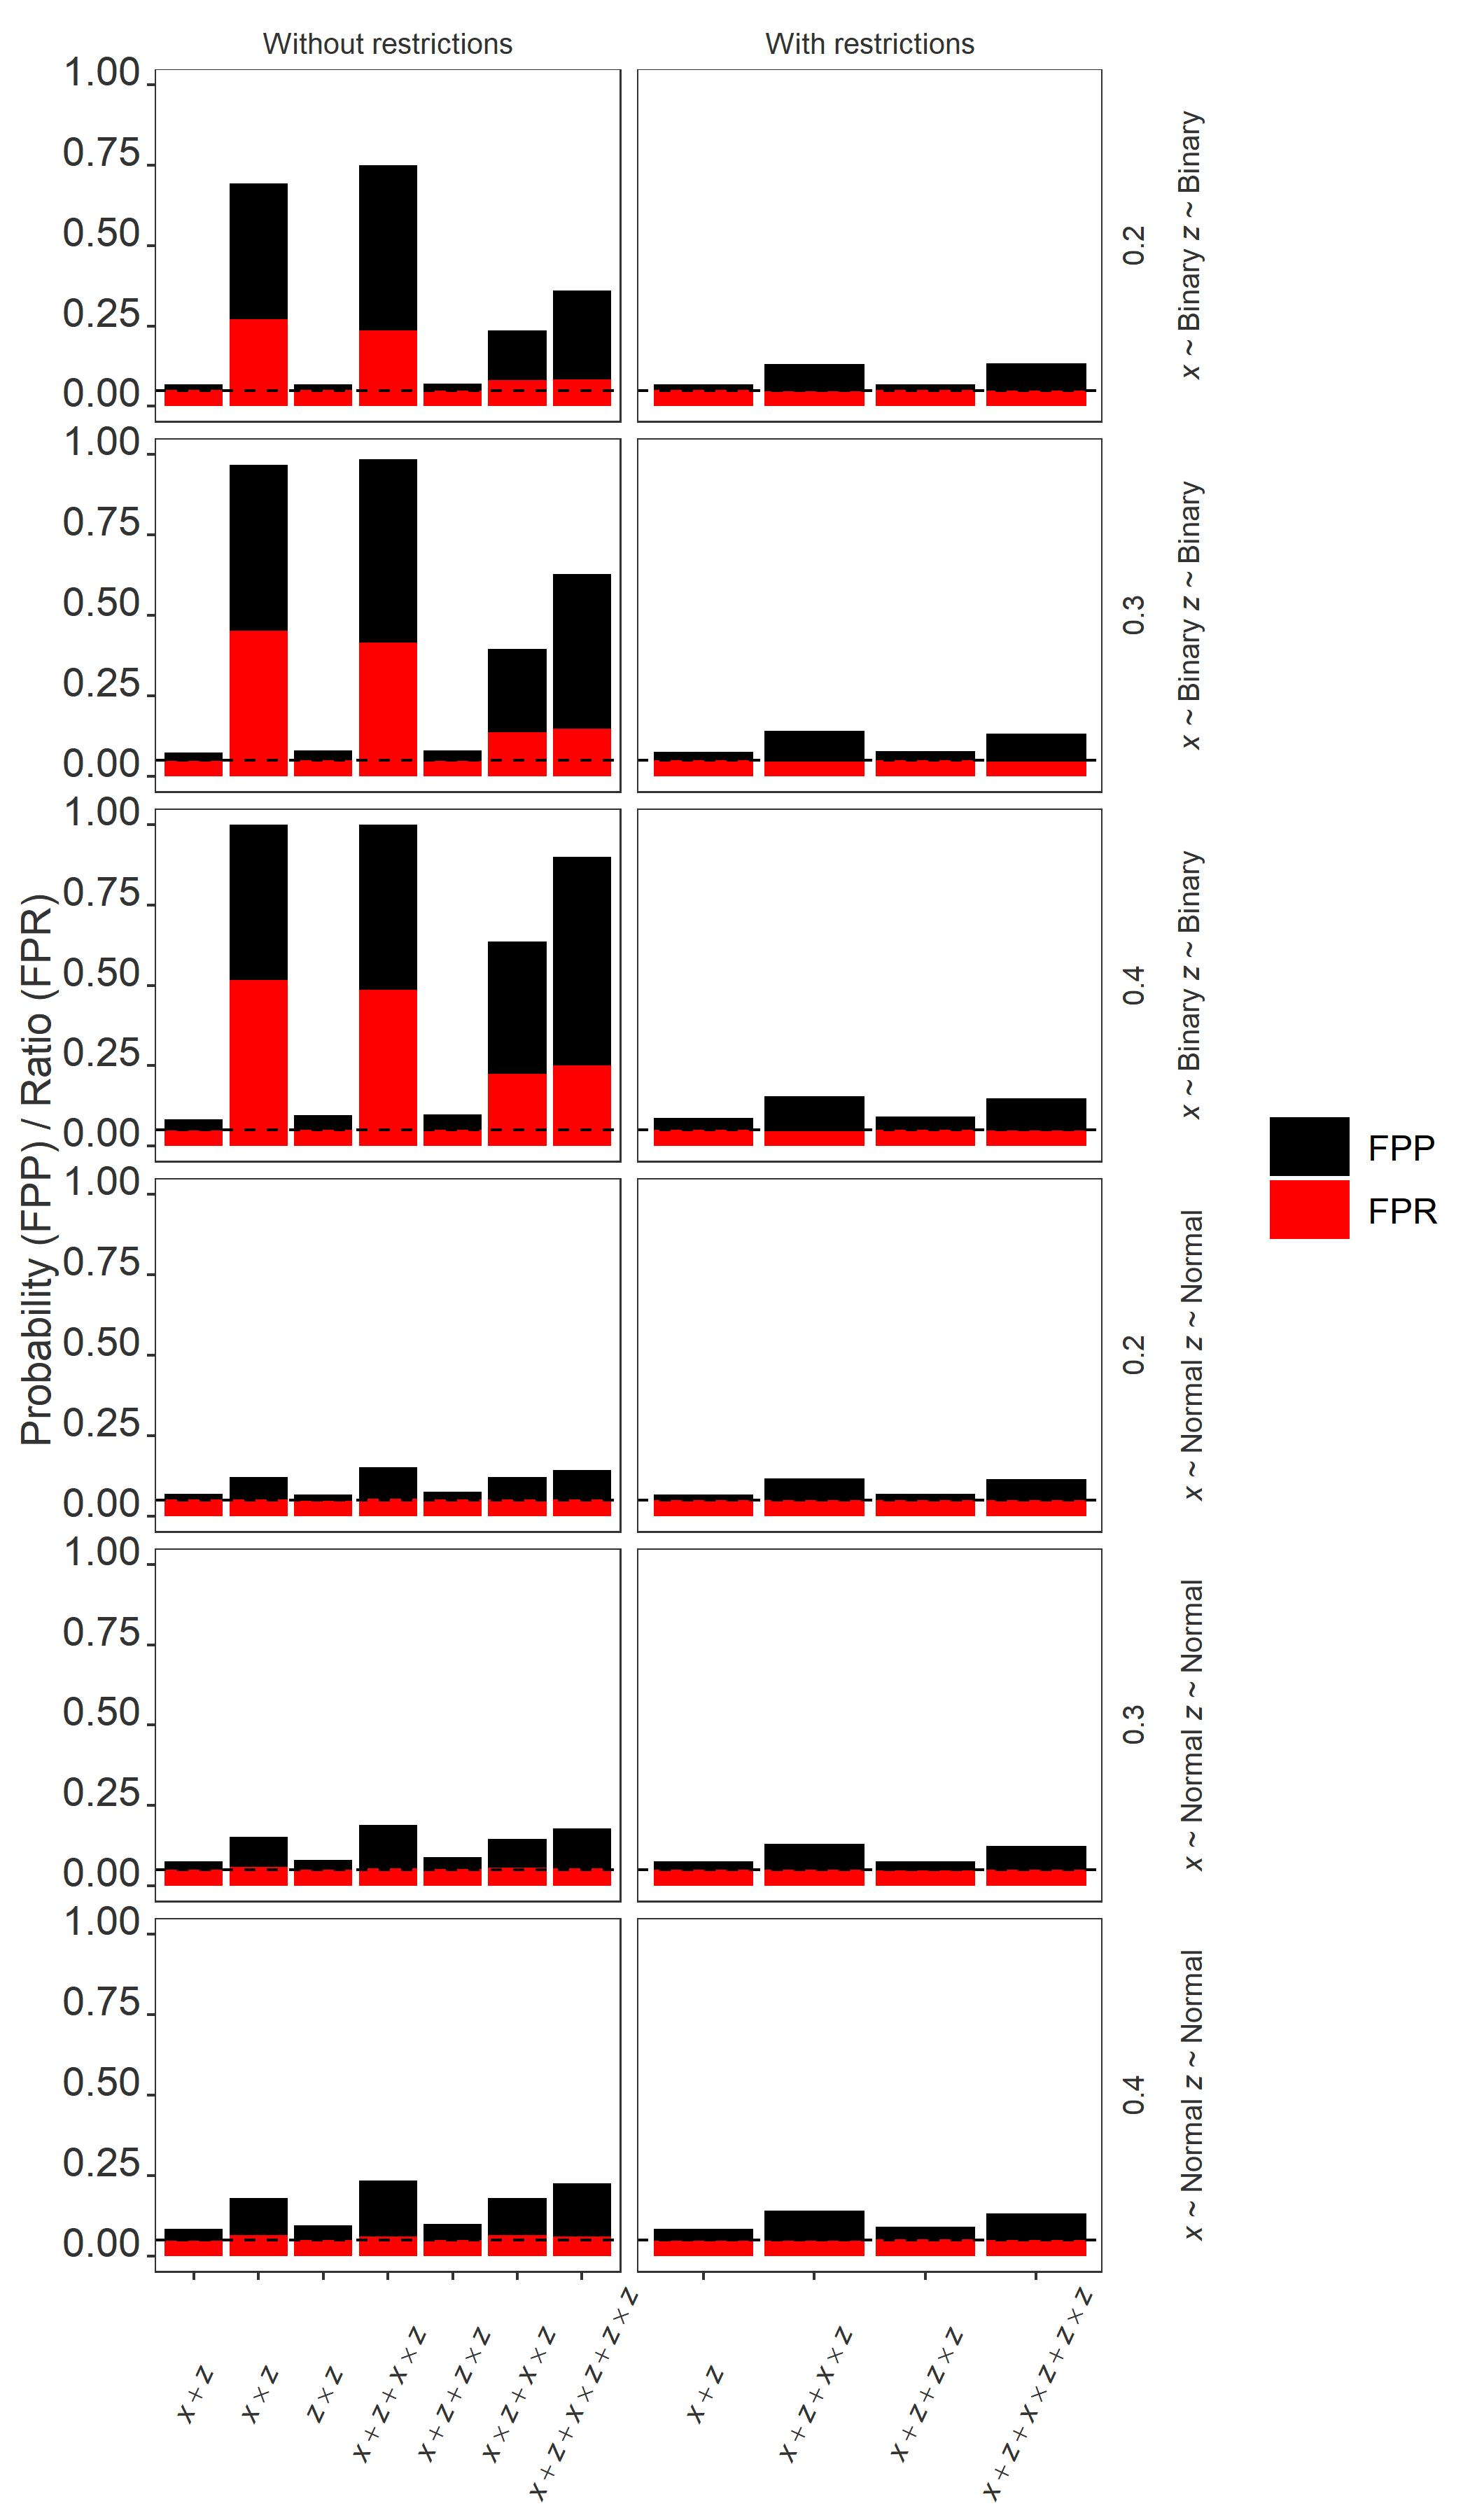
\includegraphics[scale=0.7]{R/Analysis/Result/Figures/Figure2SIBon.jpeg}
\centering
\caption{False positive probability and false positive for different levels of correlation between the dependent variable and the covariates ranging from  $\textit{r}=0.2$ to  $\textit{r}=0.4$ when using Bonferroni correction. Black denotes the false positive probability and red denotes the false positive ratio. Dashed blacked line indicates 0.05. The description of the figure is otherwise the same as for Figure \ref{fig:appfigure7}.}
\label{fig:appfigure8}
\end{figure}
\end{landscape}



\begin{figure}[hbt!]
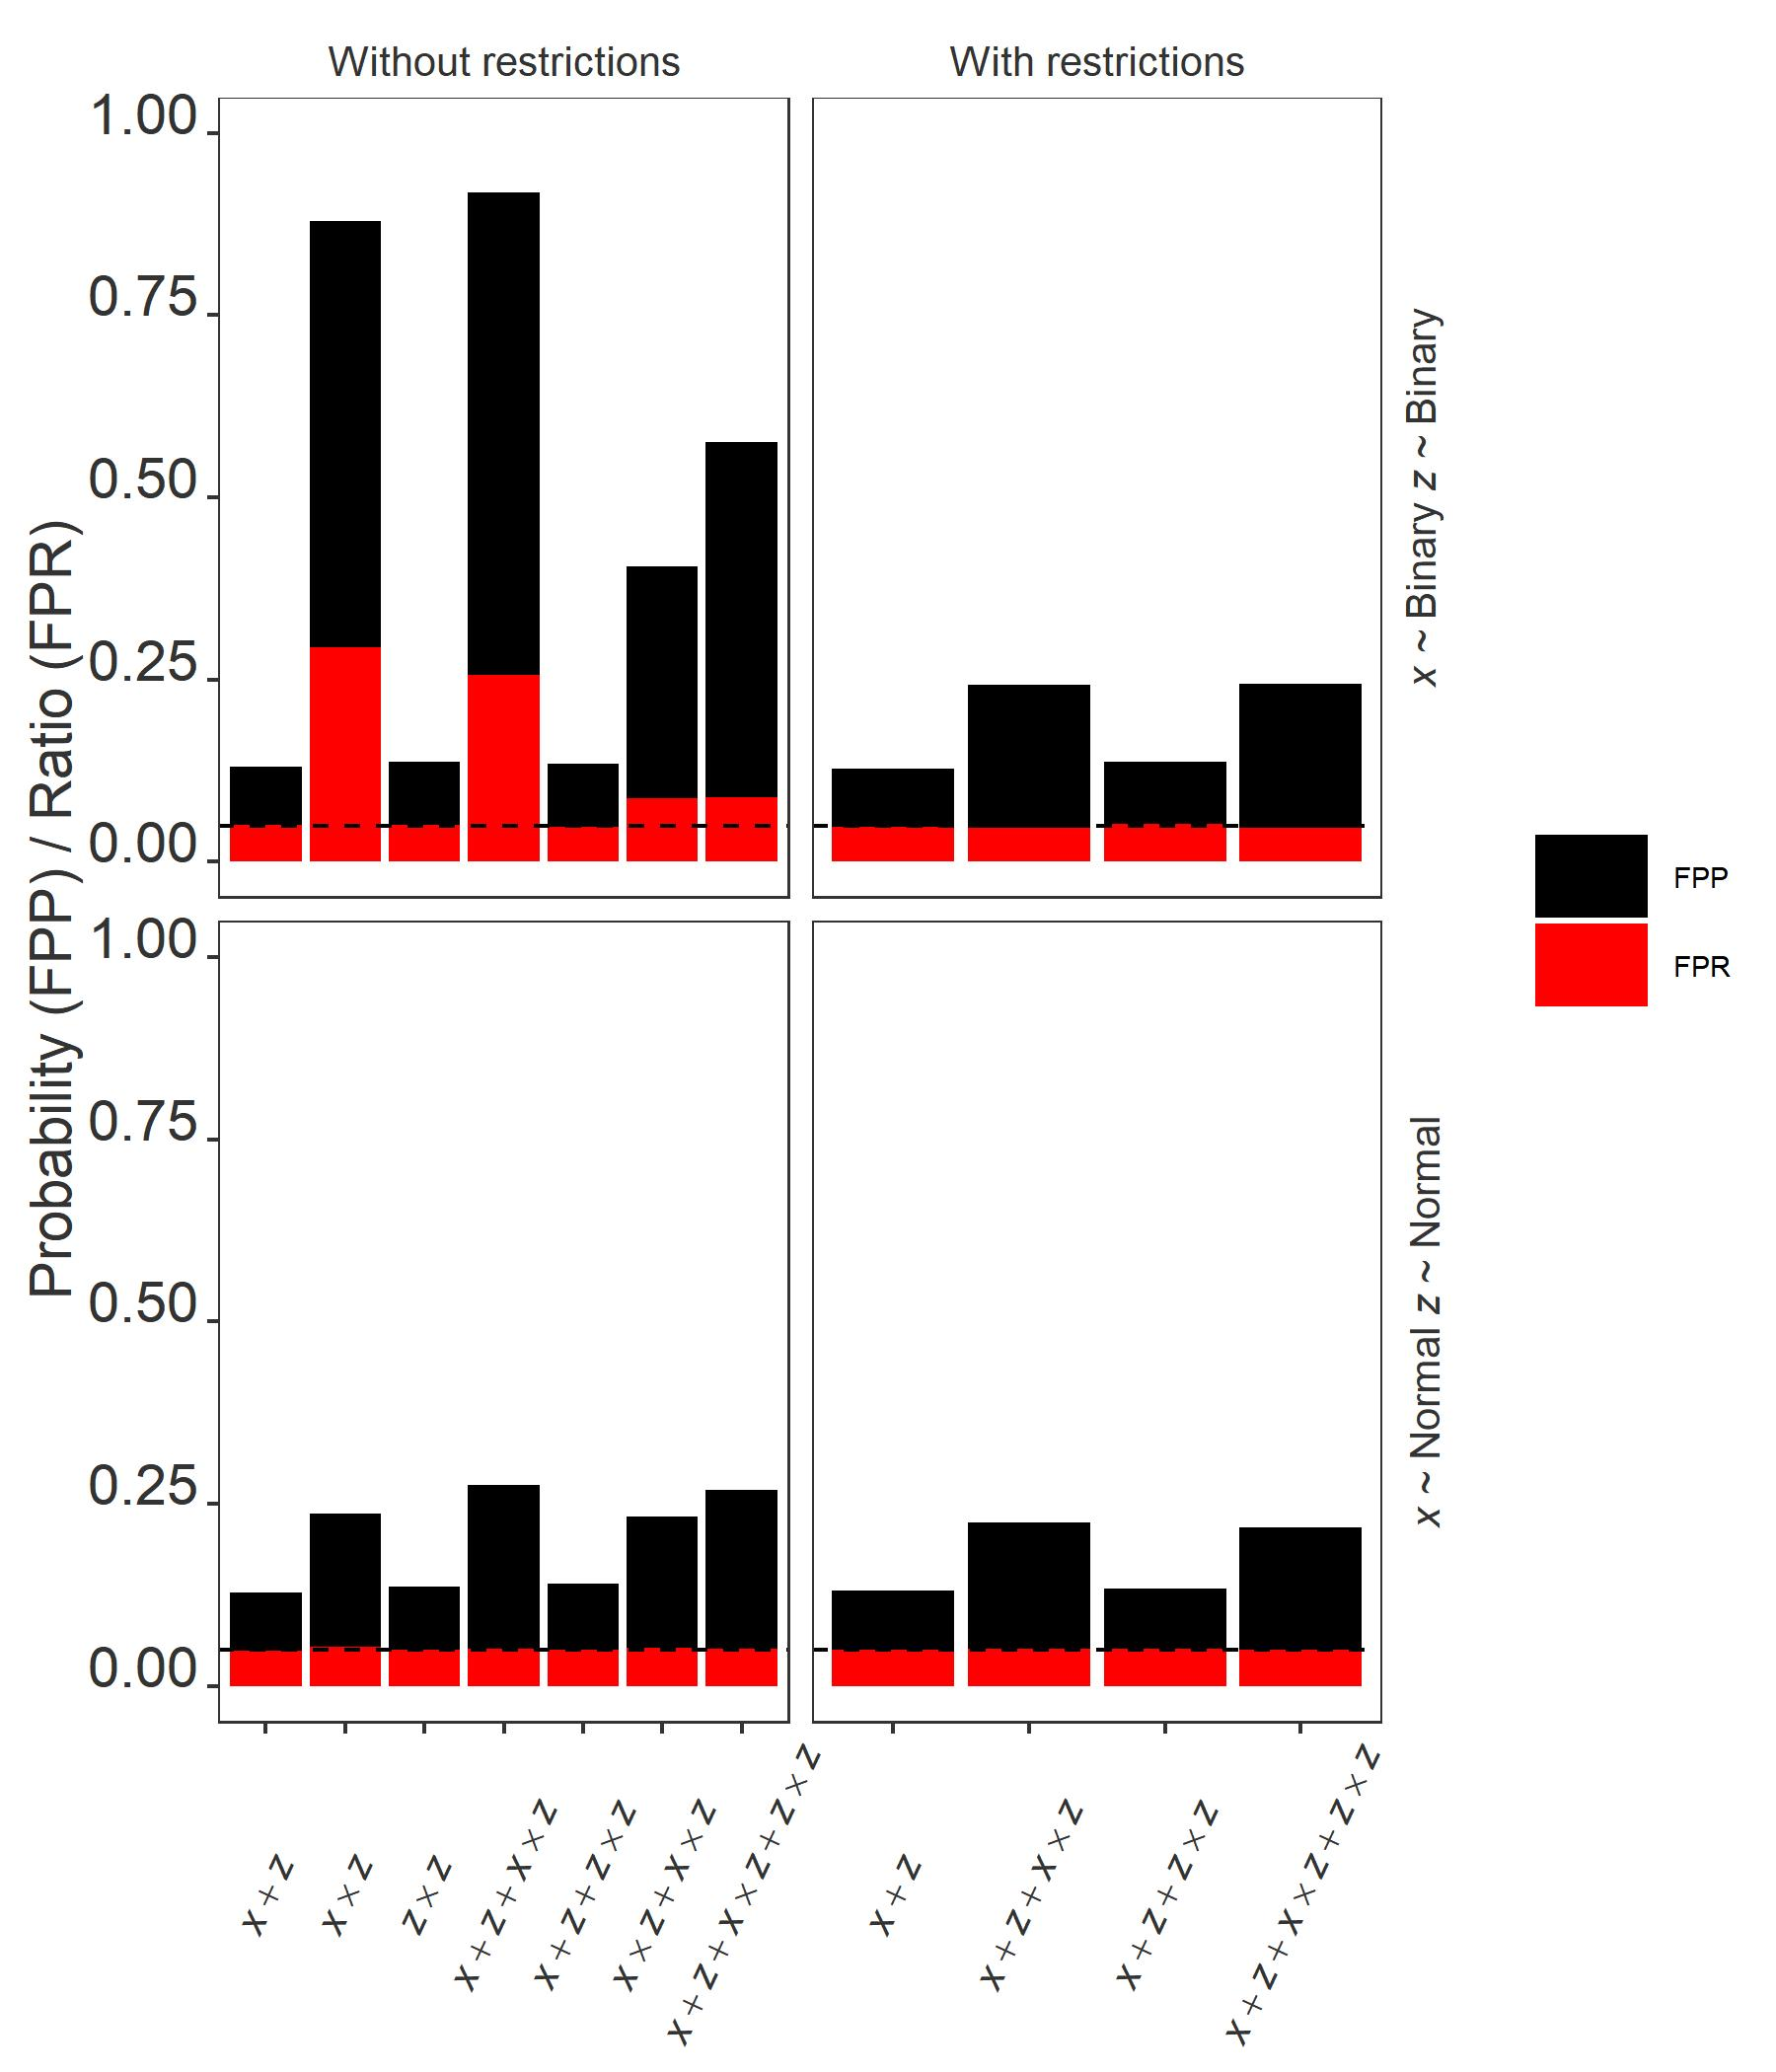
\includegraphics{R/Analysis/Result/Figures/Figure3SIBon.jpeg}
\centering
\caption{False positive probability and false positive ratio when using two dependent variables and the average of the two (meaning three dependent variables in total) when using Bonferroni correction. The correlation between the dependent variables is set to  $\textit{r}=0.5$ with the correlation between the dependent variables and covariates still at  $\textit{r}=0.2$. Black denotes the the false positive probability and red denotes the false positive ratio. Dashed blacked line indicates 0.05. The description of the figure is otherwise the same as for Figure \ref{fig:appfigure7}.}
\label{fig:appfigure9}
\end{figure}


\begin{figure}[hbt!]
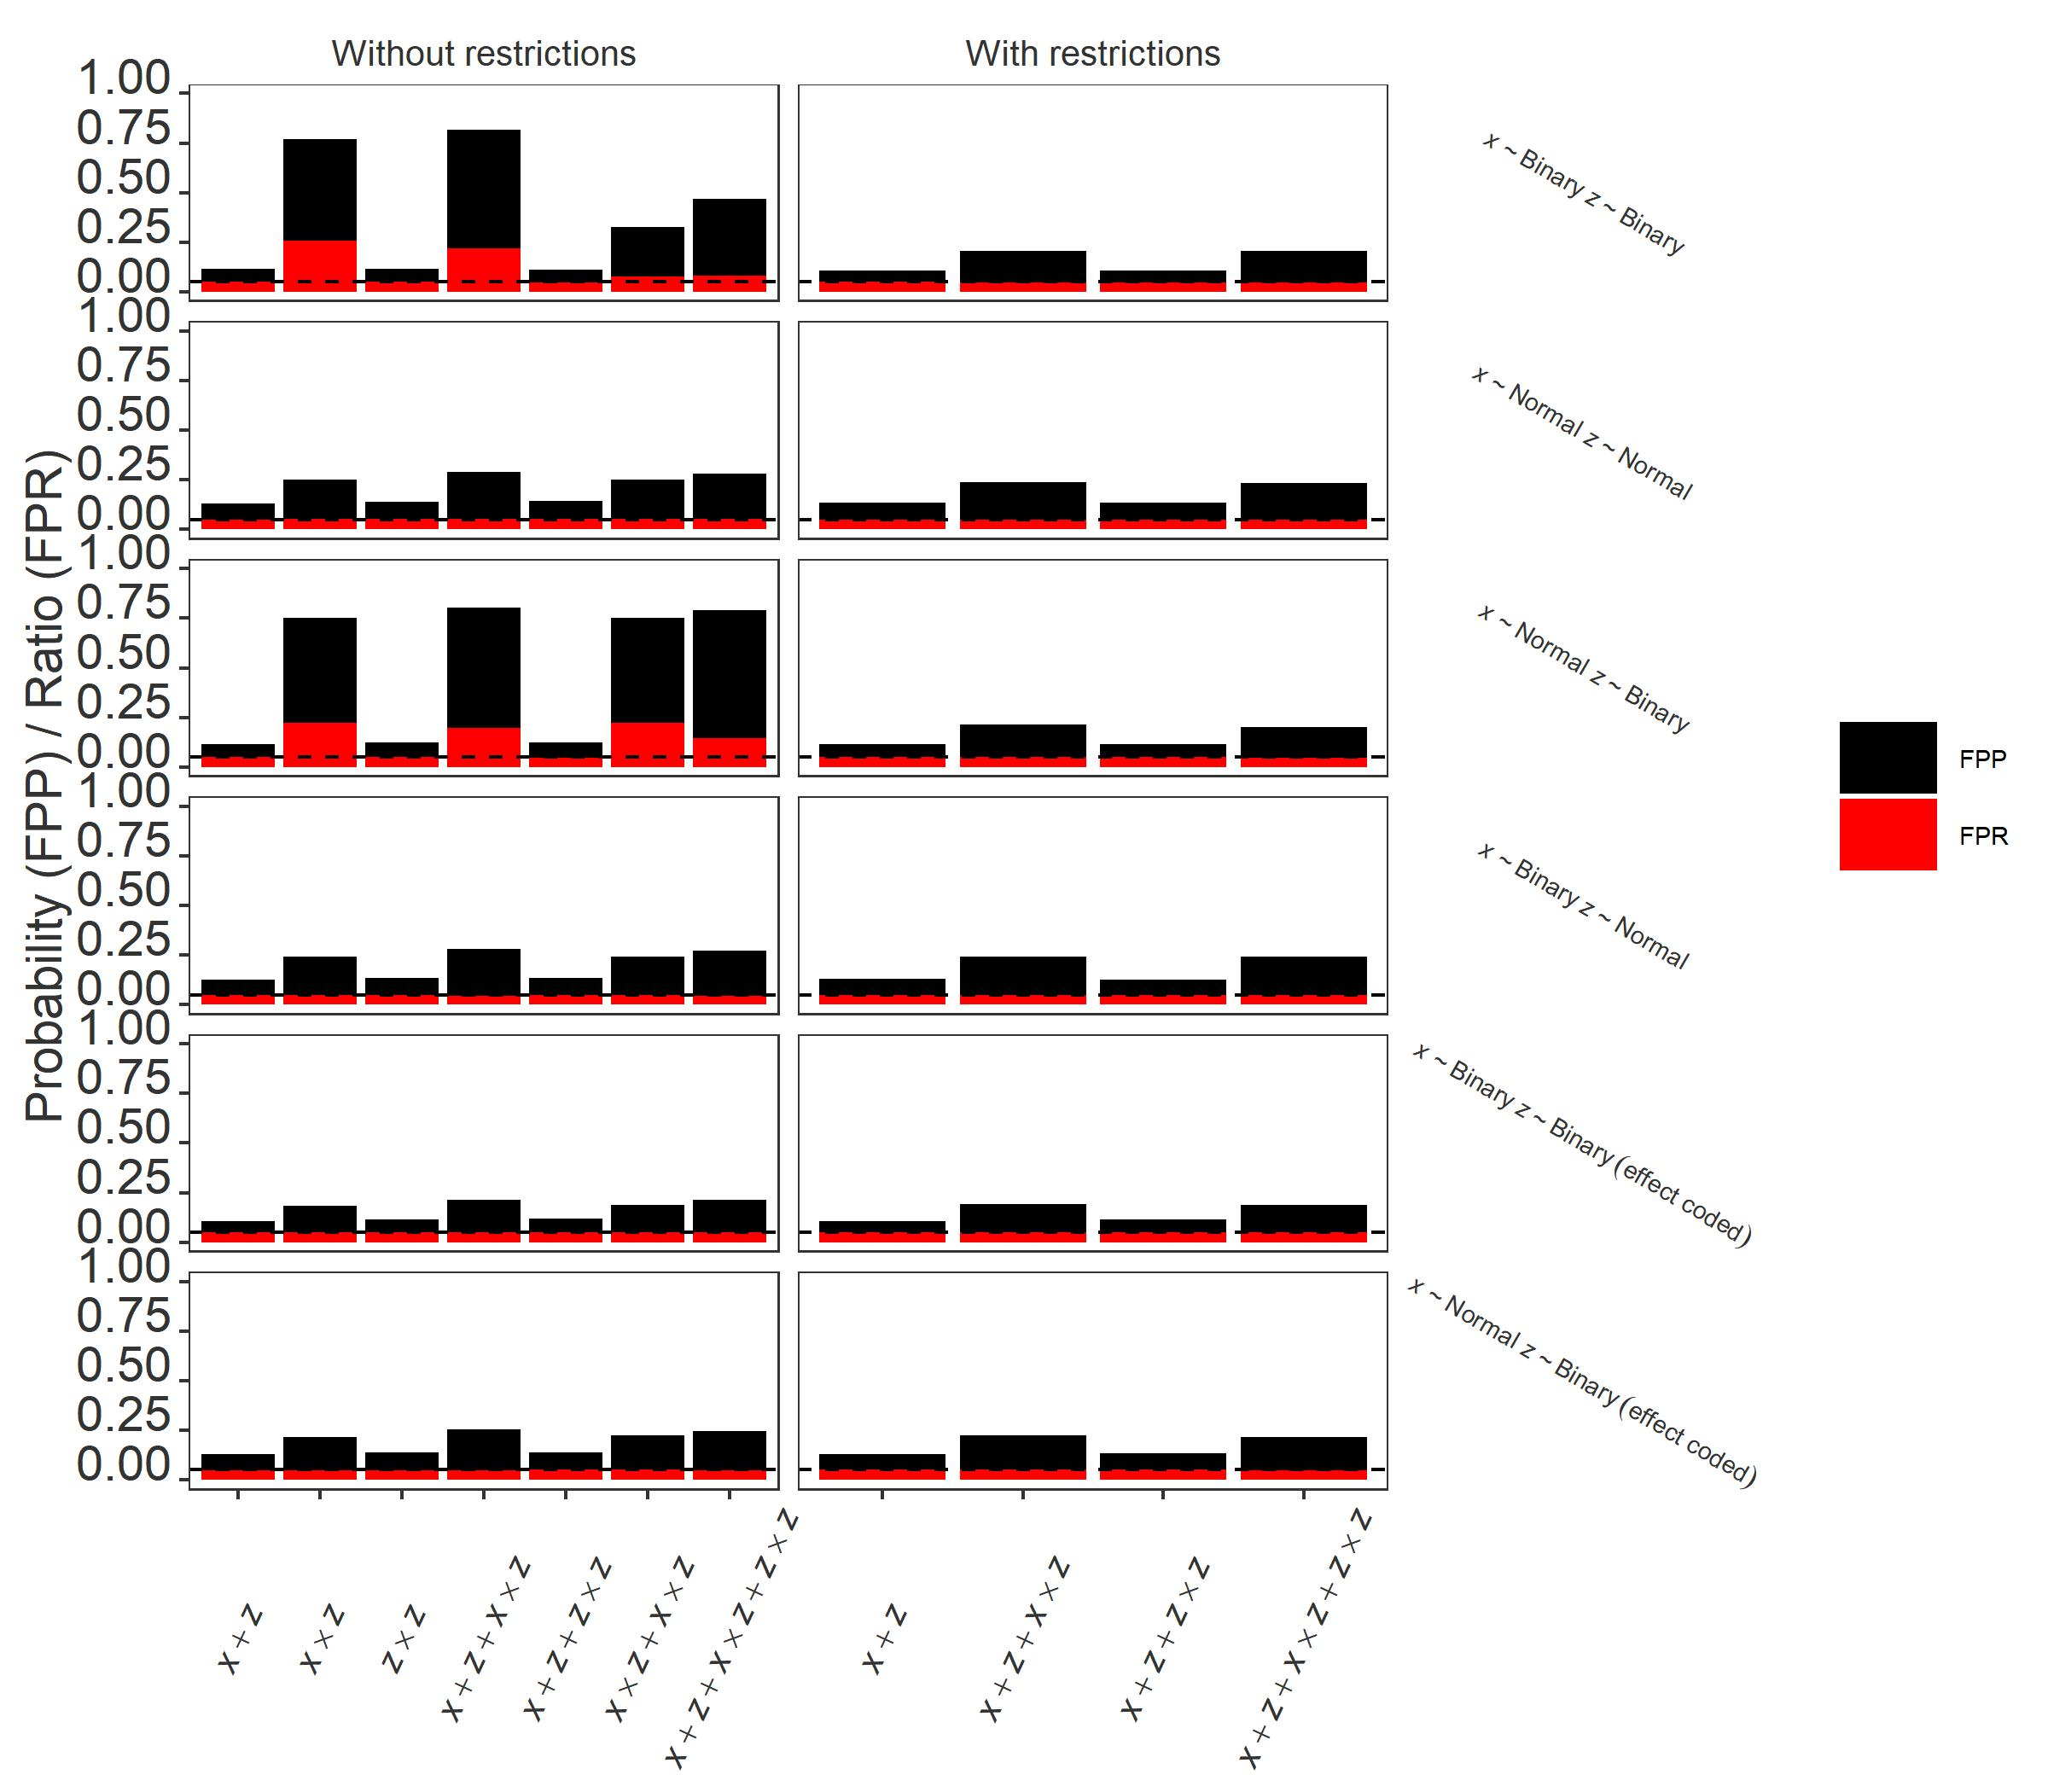
\includegraphics[scale=0.95]{R/Analysis/Result/Figures/Figure1BSIBon.jpeg}
\centering
\caption{False positive probability and false positive ratio when using multiple outlier criteria when using Bonferroni correction. Black denotes the the false positive probability and red denotes the false positive ratio. Dashed blacked line indicates 0.05. The description of the figure is otherwise the same as for Figure \ref{fig:appfigure7}.
}
\label{fig:appfigure10}
\end{figure}


\begin{figure}[hbt!]
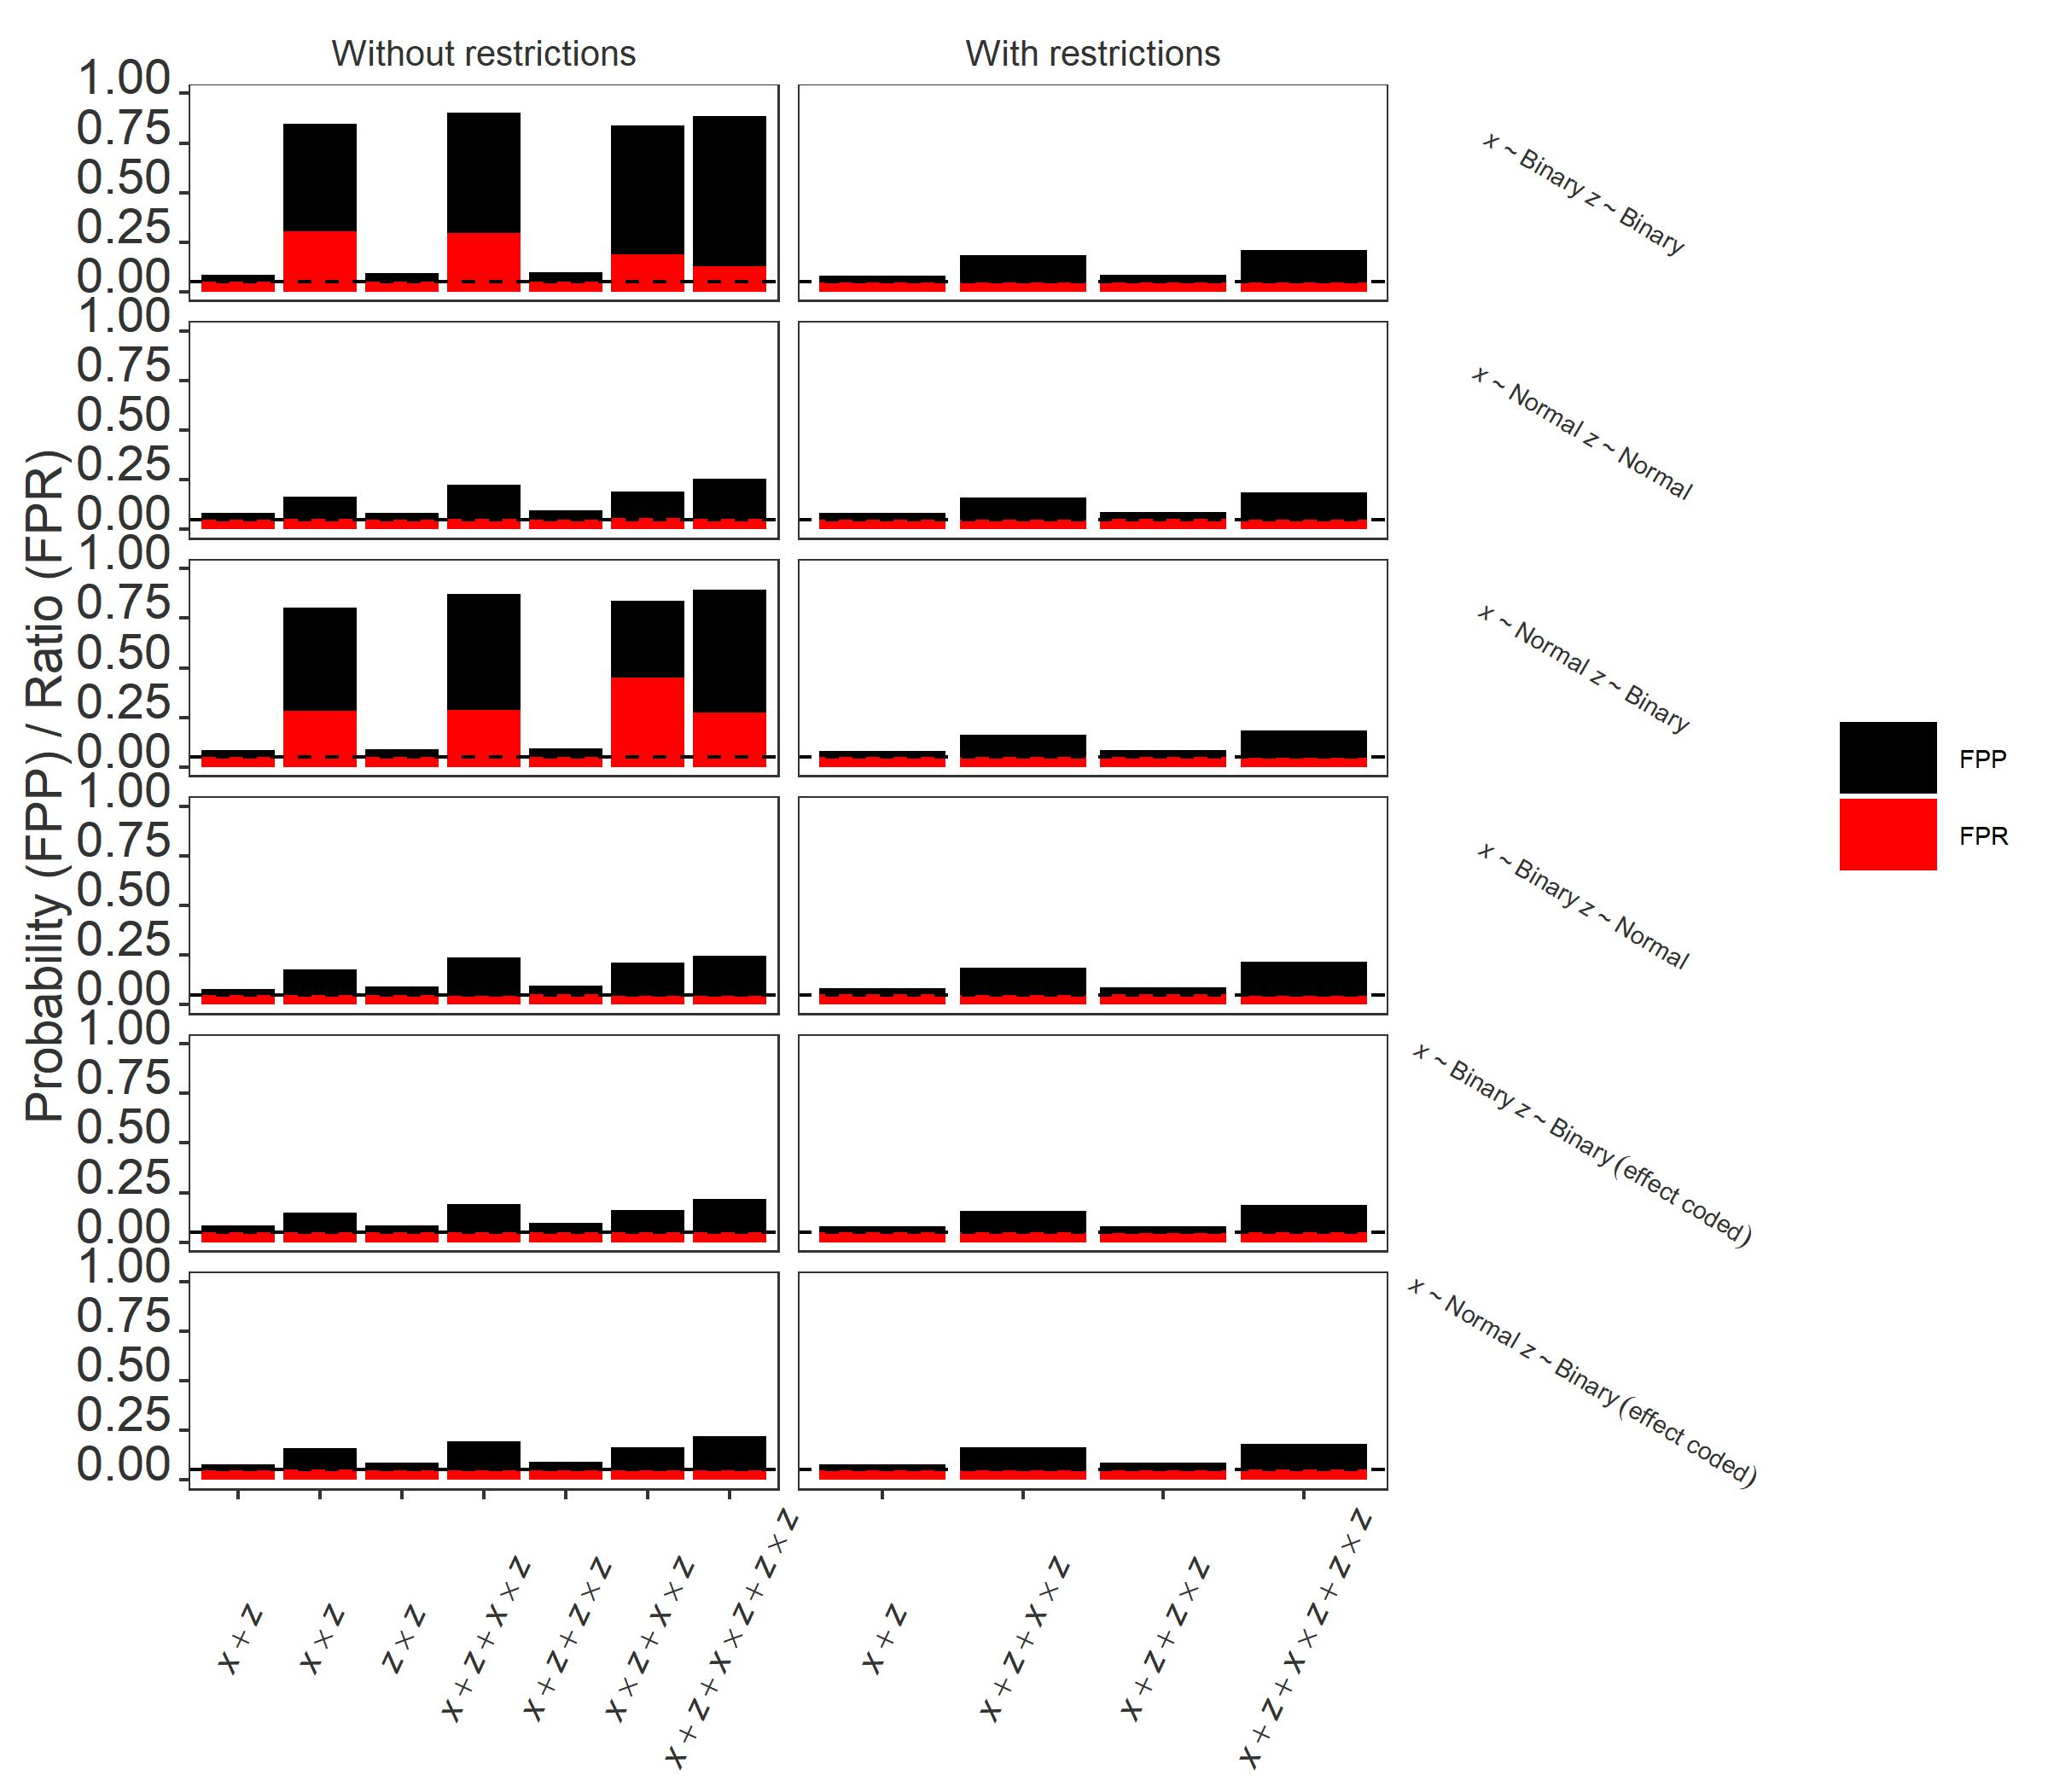
\includegraphics[scale=0.95]{R/Analysis/Result/Figures/Figure1CSIBon.jpeg}
\centering
\caption{False positive probability and false positive ratio when using three covariates instead of two as in the base line model and using Bonferroni correction. Black denotes the the false positive probability and red denotes the false positive ratio. Dashed blacked line indicates 0.05. The description of the figure is otherwise the same as for Figure \ref{fig:appfigure7}.
}
\label{fig:appfigure11}
\end{figure}


\begin{landscape}
\begin{figure}[hbt!]
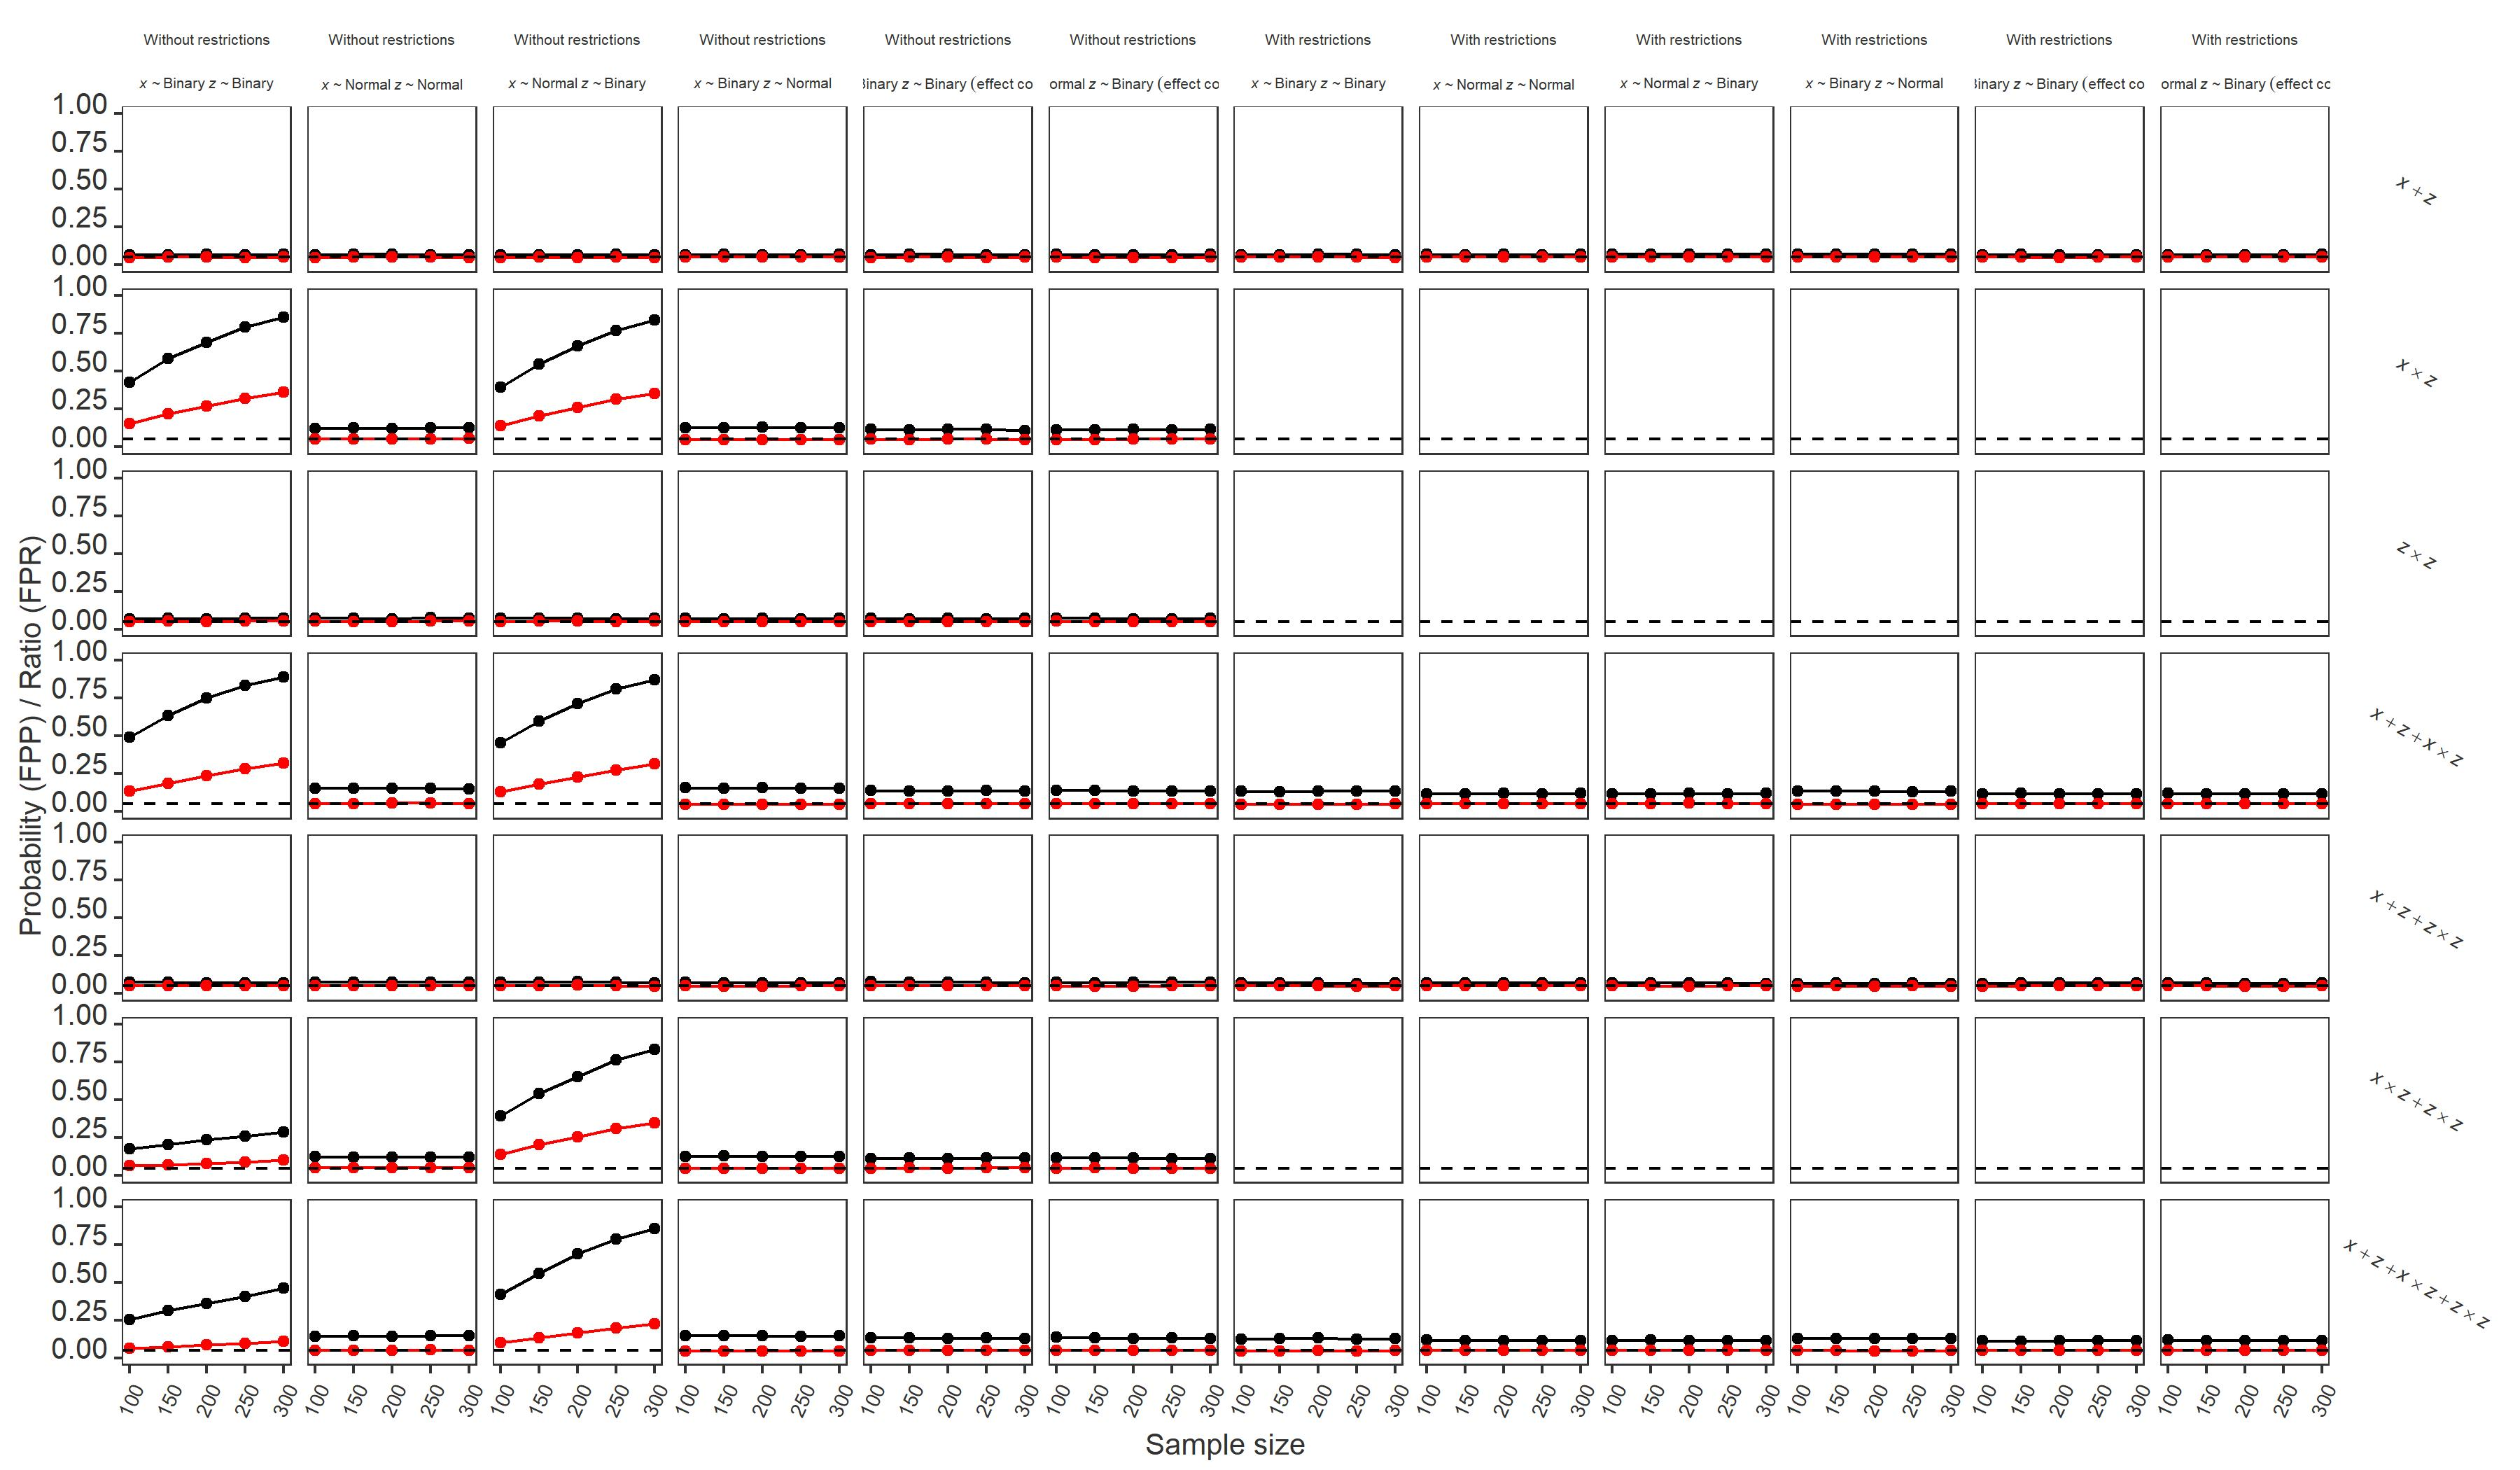
\includegraphics[scale=0.75]{R/Analysis/Result/Figures/Figure1DSIBon.jpeg}
\centering
\caption{Effect of increasing sample size for each model set and all combinations of data distributions (i.e., binary and normal) when using Bonferroni correction. Black denotes the false positive probability and red denotes the false positive ratio. Dashed blacked line indicates 0.05. The description of the figure is otherwise the same as for Figure \ref{fig:appfigure1}.}
\label{fig:appfigure12}
\end{figure}
\end{landscape}
